\documentclass[11pt]{article}

\usepackage[utf8]{inputenc}
\DeclareUnicodeCharacter{0301}{\'{e}}
\usepackage[T1]{fontenc}
\usepackage{setspace}
\usepackage{soul}

\usepackage{amsmath}
\doublespacing

\usepackage{indentfirst}
\usepackage[left=1in,right=1in,top=1in,bottom=1in]{geometry}
\usepackage[section]{placeins}
\usepackage{titlesec}
\titlelabel{\thetitle.\quad}
\usepackage{authblk}
\usepackage{csquotes}
\usepackage{booktabs}
\usepackage{siunitx}
\newcolumntype{d}{S[input-open-uncertainty=, input-close-uncertainty=, parse-numbers = false, table-align-text-pre=false, table-align-text-post=false ]}
\usepackage{amssymb}
% \newcolumntype{d}{S[input-symbols = ()]}
\usepackage{float}
\usepackage{dcolumn}
\usepackage[bottom]{footmisc} 
\usepackage[textsize=tiny]{todonotes}
\usepackage{longtable}
\usepackage{array}
\usepackage{multirow}
\usepackage{wrapfig}
\usepackage{colortbl}
\usepackage{tabu}
\usepackage{threeparttable}
\usepackage{threeparttablex}
\usepackage[normalem]{ulem}
\usepackage{makecell}
\usepackage{xcolor}
\newcommand{\red}[1]{\textcolor{red}{#1}}
\usepackage{afterpage}
\usepackage{graphicx}
\usepackage{subcaption}
\usepackage{pdflscape}
\usepackage[font=small,skip=0pt]{caption}
\usepackage{bbding}
\usepackage{xargs}
\usepackage{xpatch}
\usepackage{ragged2e}
\usepackage{rotating}
\usepackage[hyphens]{url}
\usepackage[citecolor = blue]{hyperref}
\hypersetup{colorlinks = true, linkcolor = red, urlcolor = teal}

\usepackage{comment}

\graphicspath{{~/OneDrive - University of Illinois - Urbana/Research/Projects/Sesmarias Brazil/Figures/01. Maps/}}

\usepackage{bookmark}
\usepackage{todonotes}
\setlength{\marginparwidth}{2cm}

\usepackage[backend = biber, style=authoryear, sorting = nty, maxcitenames=2, maxbibnames = 99,
uniquelist=false, sortcites=true]{biblatex}

\addbibresource{citations_sesmarias.bib}

\DeclareFieldFormat{citehyperref}{%
  \DeclareFieldAlias{bibhyperref}{noformat}% Avoid nested links
  \bibhyperref{#1}}

\DeclareFieldFormat{textcitehyperref}{%
  \DeclareFieldAlias{bibhyperref}{noformat}% Avoid nested links
  \bibhyperref{%
    #1%
    \ifbool{cbx:parens}
      {\bibcloseparen\global\boolfalse{cbx:parens}}
      {}}}

\savebibmacro{cite}
\savebibmacro{textcite}

\renewbibmacro*{cite}{%
  \printtext[citehyperref]{%
    \restorebibmacro{cite}%
    \usebibmacro{cite}}}

\renewbibmacro*{textcite}{%
  \ifboolexpr{
    ( not test {\iffieldundef{prenote}} and
      test {\ifnumequal{\value{citecount}}{1}} )
    or
    ( not test {\iffieldundef{postnote}} and
      test {\ifnumequal{\value{citecount}}{\value{citetotal}}} )
  }
    {\DeclareFieldAlias{textcitehyperref}{noformat}}
    {}%
  \printtext[textcitehyperref]{%
    \restorebibmacro{textcite}%
    \usebibmacro{textcite}}}

\renewcommand*{\nameyeardelim}{\addcomma\space}

% Makes the authors name bold in the References section:

\def\sectionautorefname{Section}
\def\subsectionautorefname{Subsection}

\title{Land Grants in Colonial Brazil and Long-Term Effects on Development\thanks{I would like to thank my committee members  Richard Akresh, Marieke Kleemans, Felipe Valencia Caicedo, and Mary Arends-Kuenning. I would also like to thank my cohort, and the seminar participants at UIUC's Applied Micro Research lunch}}

\author{Vinicius Okada da Silva\thanks{Contact information: University of Illinois at Urbana-Champaign. Department of Economics, 1407 W. Gregory Drive, David Kinley Hall: Room 126, Urbana, Illinois 61801. E-mail: vo10@illinois.edu}}

\affil{Department of Economics, University of Illinois at Urbana-Champaign}

\date{}

\begin{document}

\maketitle
\thispagestyle{empty} 

\begin{abstract}
  Legal access to land in Brazil has been a key political issue for the past century. 
  The concentration of land in large estates that are often unproductive is argued to be a factor in the rural population's low social mobility and inequality. 
  However, restricted land access in Brazil has its roots in colonial times when Large plots of land were distributed from 1530-1822 through land grants called \textit{sesmarias}. 
  Through a novel georeferenced dataset on the location of the grants in eight Brazilian states, I estimate the long-term effects of the grants on Brazil's land distribution. 
  Using propensity score matching, an instrumental variable, and exploiting colonial policy variation on where the grants could be assigned, I find consistent positive effects of land concentration in 1995 for municipalities with a colonial land grant.
  The estimates vary between 2 to 22 percentage points increase in the share of agricultural land in properties of over 2,000ha, depending on the methodology and subregion of Brazil.
  %I find that the presence of a land grant in a municipality in 1995 increases the share of farms over 2,000 hectares by 4\%.
  % Results are robust to a variety of specifications, including variations in where the grants could be assigned alongside an instrument variable approach.
  Land grants are also associated with increased land conflicts and urbanization in modern Brazil.
  %These land grants were often given to people with substantial financial means, restricting land access to most of the population. 
  %I contribute to the understanding of colonial land tenure in Brazil by collecting a novel dataset on the location of these land grants alongside a matching procedure. Results indicate that the land grants had persistent effects until the 20th century.
\end{abstract}

\clearpage
\pagenumbering{arabic} 

\section{Introduction}

\begin{displayquote}
  ``In the \textit{sesmarialismo}, thus, is the base to all of [Brazil's] land evolution"
  \\ 
  \smallskip
  - The Sesmarial System in Brazil, \textcite[p.~25]{Da_Costa_Porto1979-dz}
  \end{displayquote}

Brazil has one of the highest levels of land inequality in the world, with the USAID reporting in 2016 that 1\% of the population owns 45\% of all the land \parencite{Usaid2016-xs}. 
The issue of land inequality is compounded by the fact that large farms in Brazil are often unproductive.
The Brazilian Agrarian Reform Agency (INCRA) reported that in 2010 ``72\% of all land occupied by large holdings was considered unproductive'' \parencite{Carlson2019-mk}.
The combination of both land concentration and low levels of utilization has compounding effects on the economy as it depresses rural wages, keeping rural workers away from the consumer markets \parencite[p.~1]{De_Oliveira_Andrade1980-xz}.
% However, this is not a recent issue as even in the 1920 census, average land inequality per municipality was already high \parencite{Wigton-Jones2020-ex}. 
However, land inequality has existed in Brazil ever since its colonization, as land was distributed in large estates that were not intensely cultivated \parencite[p.~53]{Mueller1995-gi}. 

In this paper, I analyze the historical colonial causes of land inequality in Brazil by exploiting time and geographical variation in the request for land grants, called \textit{sesmarias}.\footnote{Throughout the paper, I will use land grants, grants, and \textit{sesmarias} interchangeably.}
These land grants, which in my dataset were given in the 17th to the 19th century, were often large and given to people with sufficient capital to invest in it.
I exploit the grants' geographical and temporal variation to study their long-term effects on Brazil's economic structure.  
Given the prominence of land grants in colonial Brazil and the \red{variation on why the land was granted}, this paper studies the long-term effects of the role of colonial land assignment in development using a novel georeferenced dataset on the location of the land grants in Brazil.  

\begin{comment}
\red{I further expand the models from [add the old literature] studying the relationship between land size and productivity.}
\end{comment}

\red{
I first describe how the grants were distributed and describe the process of their geographical expansion. 
Earlier grants mainly were located along the coast, and a push westward did not occur until the 1700s. 
Geographically, the grants were also often clustered near the capitals of each state.
Timewise, the distribution of the grants increased during the 18$^\text{th}$ and 19$^\text{th}$ centuries.}

I use a standard OLS alongside a propensity score matching procedure to estimate the long-term effect of the grants on land concentration. 
Both methods show a strong association between the presence of a historical land grant with a distributional shift in the concentration of land in larger farms per municipality.
\begin{comment}
The estimates indicate that the presence of a \textit{sesmaria} is associated with an increase of 3 percentage points in the share of agricultural land in farms over 2,000ha in a municipality. 
Estimates on land inequality are also higher for grants pre-1700, with estimated effects of 4 percentage points, while post-1700 grants are only associated with a 2.3 percentage points increase in the share of agricultural land in farms over 2,000 ha.
\end{comment}
Further, the effects are being driven mainly by decreases in the share of agricultural land in farms between 2 to 200ha, while the increase is seen for farms over 1,000ha.
Results are particularly pronounced in states in the Northeastern region, while the effects are present but diminished in the states of the Southeast. 
\red{Add here that the effects already exist in the 1920 Brazilian census.}

To further address the issue of endogeneity, I use an instrumental variable approach, similar to \textcite{Duranton2011-rv}. 
I use the explorer routes, called the \textit{Bandeira Paulistas}, as an exogenous determinant of the grant locations. 
The \textit{Bandeira Paulistas} were a cycle of exploration that irradiated from the city of São Paulo during the 18$^{th}$ century and opened up large portions of Southern and Western Brazil.
The explorers, callend \textit{bandeirantes}, were mainly occupied with the search for indigenous slaves and minerals, then looking for suitable land for farming. 
However, once the area had been explored and cleared of possible indigenous threats, they would often settle and claim the land. 
Given the role of the \textit{bandeirates} in further expanding Brazil's territory to the West, and their later request for land grants in the areas they have claimed to discover, that gives a possible exogenous determinant of the land grant locations in the Southeast. 
Consistent with the previous results, I find that the effects of land concentration remain in the Southeast on those municipalities that had a colonial land grant. 

Further, I exploit variation in two sets of policies in colonial Brazil to test historical hypothesis about the grants' impacts. 
First, I consider a 1701 ban on livestock grazing within 80km of the coast \parencites[p~.40]{Fausto2014-bh}[p~.198]{Simonsen2005-ps}[p~.460]{Bethell1984-of}. 
This policy generated both a time and geographical variation in the assignment of grants. 
When considering the coastal ban on livestock, the results indicate that only in areas farther than 80km from the coast \textbf{and} that received a land grant, there is an increase in the presence of livestock land usage and land inequality.
However, the results are present when considering either pre-1700 or post-1700 grants.

Second, I consider the Tordesillas Treaty, which split Brazil between Spain and Portugal until 1750. 
Using the geographical variation on the assignment of Spanish and Portuguese Brazil, I test whether the exposure to Portuguese colonization is the sufficient driver of the results of land inequality or if there are compounding effects of the grants themselves.
I find that while municipalities on the Portuguese side do have a higher share of large estates \textbf{however} the presence of grants exacerbates these effects.
Moreover, grants on the Spanish side are also associated with increased land inequality.
The results indicate that differential institutions, as measured by the Portuguese and Spanish sides, are insufficient to explain present-day variation in land inequality. 
Instead, the presence of the land grants is a key factor associated with land distribution.
%I find that the [

% Might want to move this earlier.
I also test whether there are heterogeneous effects on land concentration between Brazil's Northeast and Southeast regions. 
Given the regional disparity in development in the present, with the Northeast being considerably poorer and less developed than the Southeast, it could be argued that the land grants had a stronger effect in the Northeast.
The results indicate that the land grants are associated with increased land concentration in both regions. 
\begin{comment}
Pre-1700 increase the land concentration only in the Northeast, where they are associated with an increase of 5 percentage points in the share of farms over 2,000 ha.
Post-1700 grants, however, affect both regions similarly, being associated with an increase of 3 percentage points in the share of farms over 2,000 ha. 
\end{comment}
\red{Add here the distributional effects}
These results indicate that the grants themselves did not only have a regional impact but are also pervasive in both regions.

\red{I further test the assocation between land size and land unproducitivity in Brazil, that had been established in [add citations here]. The results match the literature, indicating that municipalities that did receive a grant only see less usage of land in the large plots, while the effects are zero or negative for smaller plots [have to add here definition of large and small plots].}

I then turn to understand the mechanisms that drive the results. 
First, I test through satellite data whether the grants are associated with urbanization and whether there are effects on land tenure and security.
\red{
I find that grants pre-1700 are associated with an increase in urbanization and are not associated with land squatting or misuse of land.
I also test the relationship between the land grants and land conflict.
I find that the presence of a grant, whether pre-1700 or post-1700, is associated with an increase in land-related conflicts between 2014 and 2018.
Lastly, I measure the effects of the grants in the presence of slavery in 1872 through a novel georeferenced dataset at the parish level. 
The results indicate that only the earlier grants, pre-1700, were associated with a lower presence of slavery.}

The first contribution of this paper is through the historical data colelcted.
This paper provides a novel georeferenced dataset of colonial land grants in Brazil for seven states in the Northeast and Southeast.\footnote{The list of states is Alagoas, Paraiba, Pernambuco, Rio Grande do Norte, Bahia, Minas Gerais, and Sao Paulo.}
Through archival work and collaboration with Brazilian researchers, over 4,000 land grants were successfully georeferenced, providing a novel dataset that allows researchers to study and understand the patterns of colonization in Brazil.
%The eight states in which this work is focused constitute X\% of the total area and X\% of the population of Brazil.
Further, these states analyzed in this paper were also historically where colonization began, making the study of the colonial past especially relevant.\footnote{Further work must be done to collect and georeference data for the rest of Brazil.}
\red{I further contribute by providing the first georeferenced dataset for 1872 and 1890 parishes, which allows for more precisely geographical measures} 

Second, this paper contributes to the further understanding of colonial institutions and their long-term effects on development \parencite{Engerman2002-ju, Acemoglu2005-ti, Eslava2023-eq, Bruhn2012-cc}. 
Previous studies in Latin America have studied the institutions of the \textit{mita}, \textit{haciendas}, and \textit{concertaje} in Spanish America, such as \textcite{Dell2010-qt}, \textcite{Faguet2022-sr} and \textcite{Rivadeneira2024-uj}.
While the \textit{sesmarias} are similar to the \textit{haciendas}, their size and the fact that they were often freely distributed to wealthy people in colonial Brazil gives a different contrast on how they could affect long-term development.
This paper adds to the literature by studying a key institution that prevailed in Brazil for over 200 years, the \textit{sesmarias}.

Third, there are no empirical papers studying the direct causes of colonial land distribution in Brazil. 
Previous literature has found negative long-term effects of colonial land usage in Africa and South America \parencite{Dell2010-qt, Lowes2021-ww, Montero2022-ua}. 
However, there exists evidence that not all colonial land regimes led to negative effects and instead led to economic development, with examples in India and Indonesia \parencite{Banerjee2005-ki, Dell2020-zo, Ratnoo2023-vw, Caum-Julio2023-ei}.  
Other studies have analyzed the effect of land grants in the United States \parencite{Akee2014-uw, Allen2019-kh, Smith2023-ip}. 
Other works have analyzed land distribution and reforms in Europe \parencite{Reed2012-qy, Goni2022-do}.
By studying Brazil, one of the countries with the highest levels of land inequality in the world, I conduct the first empirical study analyzing the historical roots of land inequality in the country.

\red{Probably want a paragraph studying the effects of land inequality.}
\red{Land Inequality in Italy \parencite{Bianchi-Vimercati2022-jy}}

This paper also contributes to the understanding of Brazil's historical economic development by explaining the diverging paths in development in each region. 
The land regime and size in each region, as measured by the land grants, could have differential impacts on development.
\textcite{Wigton-Jones2020-ex} studies the effects of 1920 agricultural census land inequality and how it still has persisted to the present.
The literature has analyzed how different economic cycles and how immigration led to differential educational outcomes in Brazil \parencite{Musacchio2014-pq,Rocha2017-yq, de-Carvalho-Filho2012-pc}.
\textcite{Ehrl2019-zp} further studies the persistence of occupations from 1872 to the present.
Related literature has also analyzed the effect of the Spanish-Portuguese borders in South America, the role of sugarcane, and gold mining in Brazil \parencites{Laudares2023-wl, Naritomi2012-or}.
Part of the literature has studied the role of pre-colonial institution and the development in Latin America \parencite{Caum-Julio2023-ei, Maloney2016-qv}.
This paper adds to the literature by focusing on a specific Portuguese institution, the \textit{sesmarias}, to study how it affects present-day Brazil.
%\parencite{Summerhill2010-yl}[No effect on...]
%\textcite{Ratnoo2023-vw} [Paper about land tenure in India]
%\textcite{Galor2009-bc}
%\textcite{Albertus2018-bf}

%\textcite{Alston2012-lz}
%\textcite{Eslava2023-eq} [Land Inequality Being Bad in Latin America]

The paper is divided as follows. In \autoref{sec:historical_background} I briefly describe the history of land in Brazil, from its colonial times to the present-day system. 
In \autoref{sec:data} I describe the land grant dataset, its collection, and the other datasets used. 
%In \autoref{sec:theory}, I provide a theoretical framework discussing the effects of land size and productivity.
In \autoref{sec:selection}, I quickly describe the evidence of the geographical selection of the land grants in Brazil.
In \autoref{sec:identification}, I discuss the four main identification methods used in the paper.\footnote{In \autoref{sec:ols}, I show both OLS and matching estimates of the long-term effects.
In \autoref{sec:iv} I discuss the instrumental variable and discuss its results.
In \autoref{sec:coastal} and \autoref{sec:tordesillas}, I exploit two sources of variation to study the differential effect of the grants.}
In \autoref{sec:challenges}, I discuss the main concerns in studying the long-term effect of land grants in Brazil. 
In \autoref{sec:results}, I discuss the results of all the empirical approaches.
\autoref{sec:mechanisms} discusses potential mechanisms and other channels through which there are persistence effects.
I discuss a few robustness checks in \autoref{sec:robustness}.
Lastly, \autoref{sec:conclusion} concludes the paper.

\section{Historical Background}
\label{sec:historical_background}

\subsection{Land Grant Implementation in Brazil and Colonization Patterns}

\begin{comment}
\hl{Tem que falar sobre as Capitanias Hereditarias e como as sesmarias tinham que ser doadas ja nessa epoca.}
\end{comment}

% \hl{Conflict and land quality ``Stanley Stein, que se dedicou ao estudo da expansao e declinio da cafeicultura em regiao de Vassouras, municipio fluminense cujo auge de producao ocorreu na decada de 1850, verificou que, enquanto se manteve elevada a disponibilidade de areas de terras devolutas e nao existia cultura economicamente remuneradora que provocasse alta dos precos da terra, poucas eram as dificuldades entre sesmeiros e posseiros" {\parencite{Nozoe2006-hj}}}

% Kind of don't like this sentence below
Portuguese presence in Brazil began in 1500, when the process of Brazil's colonization began. 
Early on, to deal with the costs of managing an overseas empire, the Portuguese Crown decided to split the country into fifteen tracts of land called \textit{capitanias}, each given to a set of powerful individuals from Portugal [cite something here].
One of the key aspects of this division, however, was that each captain was supposed to distribute the land as \textit{sesmarias} as a form of settlement. 
When Portugal abolished the system of the \textit{capitanias} it kept the distribution of the land grants.\footnote{Some municipalities were directly created and first settled because of the land grants. For example, the municipality of Taipu in the state of Rio Grande do Norte is described as being ``first settled because of a land grant in 1608''. In total, 17 grants were given to this municipality, which was a primary cause of its creation. \red{Want to add here how that matches my data, since I'm bringing this up}. More information is available (in Portuguese) at \url{https://www.taipu.rn.leg.br/a-cidade/}.}

The Portuguese Government tried to implement in Brazil a similar system of land distribution they had successfully done in the Azores and Portugal.
\begin{comment}
\red{[Add here that it was established in 1375 in Portugal because of the Black Death and the need to repopulate the countryside \parencite{Nozoe2006-hj}]}
\end{comment}
According to \textcite{Smith1944-oi}, the only way Portugal knew how to distribute the lands in Brazil was through the large \textit{sesmarias}.
However, while the legislation for granting the land was the same, two main issues differentiated how it was applied in Portugal and Brazil. 
Portugal, as a smaller state, the \textit{sesmarias} led to small properties. 
Meanwhile, in Brazil, by the need of colonization and the large area of the country, the implementation of the \textit{sesmaria} system led to the creation of larger estates than the ones seen in Portugal \parencites[p.~58-59]{Da_Costa_Porto1979-dz}[p.~28]{Diffie1987-bw}[p.~23-24]{Panini1990-rj}.

While technically, anyone could apply to get a land grant, the requirement to develop the land often led people of sufficient wealth to apply.
In practice, that led to the applications being done only by a select few who had either the money or political connections \parencites[p.~434]{Diffie1987-bw}[p.~80]{Bradford_Burns1993-nw}.
In the letter descriptions, the applicants would boast about their wealth and connections in order to be able to get a grant \parencite[p.~36]{Lima1954-td}. 
% Land belonged to the state until apportioned, or until seized through squatter sovereignty with the hope of recognition by the state at some later date. Both Portuguese and Spanish colonization entailed immediate concessions of land. In the Portuguese case, the sesmaria was for a privileged few [p. 434].
Those applicants that had the financial means to get a land grant would often get large estates, ``customarily one to three leagues in extent (16.7 to 50.1 square miles)'' \parencite{Dean1971-iq}.\footnote{Approximately 4,300 to 13,000ha.}

Given that the grants were distributed to only a few people with sufficient capital, it would generate the first division of wealth in Brazil's colonial society.
\textcite[p.~36]{Lima1954-td} indicates how those people would become the ``future sugar engine owners and farmers that would create the economic aristocracy of the colonial society''.\footnote{Additionally, \textcite[p.~47]{Lima1954-td} states that the ``The \textit{sesmaria} is the large estate, inaccessible to the farmer without resources.''} 
Further, those who did not have the means to get a land grant would often be marginalized in colonial society \parencite{Simonsen2005-ps}.
Contemporary evidence from the French botanist Augustin Saint-Hilaire describes how ``the poor that couldn't have titles, establish themselves in the land that they don't know if it is owned; they plant, build small houses, raise chickens, and when the least expected, a rich man appears with a title, expels them and enjoys the fruits of their labor'' \parencite[p.~143]{Da_Costa_Porto1979-dz}.\footnote{More evidence from the issues of squatting is further described in the letter by two grantees em 1702, who requested land alongside a river but claims people were living there without a \textit{sesmaria} grant \parencite[p.~142]{Da_Costa_Porto1979-dz}. In the interior of the Northeast when the land was full of squatters or bandits, they would often grant them away \parencite[p.~88]{Poppino1968-ab}.}
The presence of the grants land led to land concentration through the consolidation of land in the hands of owners that successfully developed their land \parencite{Manchester1931-zw}.

\begin{comment}
\red{Need more in-depth discussion of the history here}

\red{Political Effects}: \parencite{Leal2012-gj}.

\red{History of land inequality being bad in 1920 \parencite[p.~124]{Bertola2017-hr}}
\end{comment}

% Casos destes viu-os, com frequencia, Saint-Hilaire, em suas viagens pelo interior: 'os pobres, que nao podem ter titulos, se estabelecem nos terrenos que sabem nao terem dono; plantam, constroem pequenas casas, criam galinhas, e, quando menos esperam, aparacem-lhes um homem rico, com o titulo que recebeu na vespera, expulsa-os e aproveita o fruto de seu trabalho' [p. 143]

% \parencite{Simonsen2005-ps} - ``the ones that don't possess sesmarias or can't own land are disowned by the own society they live in"

% \textcite[p.~58-59]{Da_Costa_Porto1979-dz} ``Enquanto, no Portugal de D. Fernando, de D.João e de D. Duarte, a distribuição de terra de sesmaria gerou, em regra, a pequena propriedade, no Brasil foi a causa principal do latifúndio"

% Some about the dynamics of power and how squatting was risky:
% Ordinarily, however, when it was learned that a section of the sertao was infested with bandits or that an appreciable number of squatters had settled there, the area in question was awarded in a huge tract, or sesmaria, as a veritable feudal domain to a powerful cattleman (p. 88).[Poppino]

%\parencite{Carlson2019-mk}
%``For many Latin American scholars seeking to explain their region’s backwardness in the first half of the  twentieth century, the prevalence of latifundio-dominated agrarian structures was key. The latifundio was  seen  as a  fundamental  impediment  to  economic  development  due  to  its  feudal-like  social  relations,  its   tendency for monocropping, and its negative impact on the formation of domestic markets. However, it  was these scholars’ emphasis on the labor regimes that were characteristic of the latifundio that prevented  them from fully grasping the nature of the problem.''

%\parencite{Carlson2019-mk}
%``Going back to colonial times, land in Latin America has often been acquired outside of market mechanisms.  This typically occurred through massive land grants from the crown such as the merced, or the sesmaria in  Brazil, or, after independence, through free or low-cost land concessions from national or local governments  (Furtado  2003,  68–80).''

%\parencite{Carlson2019-mk}
%``Not only do extensive activities predominate, but land use statistics reveal the low-investment and low- productivity nature of these types of production. On grazing land, for example, if we divide the total number  of animals on large farms by total hectares of pasture, Brazil’s large farms have only 0.65 animals per hectare  of grazing land, while in Peru it is an incredibly low 0.06 animals per hectare (IBGE 2012; INEI 2012).''

%\parencite{Carlson2019-mk}
%``As Edelman (1992, 22) explains: “the important point is that the dynamics of accumulation are radically different than those of classical capitalist development. Rather than investing heavily in improved  technologies,  employing  productive  human  labor,  attempting  to  capture  increased  market  shares,  or   developing linkages with other production processes, latifundistas could become wealthy from harvesting  natural and quasi-natural products of the land.”''

%\textcite{Diegues_Junior1959-ba}

% \textcite{Smith1944-oi} ``The only way to distribute the lands was by grants of large tracts as sesmarias''

% \textcite{Dean1971-iq} - ``Anyone who claimed to have the means and desire to make use of the land was given a grant, customarily one to three leagues in extent (16.7 to 50.1 square miles).''

%\textcite[p.~113]{De_Oliveira_Andrade1980-xz}
% ``Extensive cattle raising, with open grazing, did not require much attention or labor. For that reason, the number of slaves in the region was small''

%\textcite[p.~119]{De_Oliveira_Andrade1980-xz}
%``[The cotton] advantage was a stimulus to the large landowners of the region, since they could increase their profits without modifying their traditional economic activities, and without forsaking cattle raising. Even today one can see that in the Agreste and Sertao cattle raising is the economic activity most associated with the latifundia. The large landowners are always principally cattle raisers and only secondarily farmers. This pattern is broken in the wet areas where climatic conditions are less favorable to cattle raising and where land is almost always in small holdinds''

%This paper describes the history of land usage in Brazil and discusses the roles of the sesmarias in it \parencite{Reydon2015-ff}.

%\textcite[p.~157]{De_Oliveira_Andrade1980-xz}
%``Cattle raising is today, as in the past, the source of great wealth in the Sertao [...] The system of cattle raising on the large fazendas of the Sertao has changed little in recent years''

%``The slaves in Brazil were at least partially integrated into society and possessed rights, quite a legal contrast to the plight of the slaves in the United States. Hence, their transition from slave to freedman was facilitated. One paramount privilege the slaves enjoyed was their ability to purchase their freedom. Blacks, taking advantage of the many Catholic holidays to work on their own, saved money for that purpose. They occasionally formed their mutual aid societies to facilitate their purchase of freedom.''

\subsection{End of the Land Grants and the 1850 Land Act}

On the brink of Brazil's independence in 1822, land concentration in Brazil was high due to the land grants throughout its colonial period \parencite{Smith1972-dv}.
Contemporaries describe that a key issue of the \textit{sesmaria} system was that a lot of the land had already been given, which led to a lot of poor families who were not able to claim land \parencite[p.~42-43]{Lima1954-td}.
As a push against the grants and the issues they were causing, in 1822, the Emperor of Brazil banned the system of \textit{sesmarias} in Brazil.\footnote{Surprisingly, in the dataset, I still observe grants being given post-1822, possibly indicating that the law was not immediately binding.}
What followed was 50 years of confusion, during which time there was no legal way to obtain land. 
As a result, squatting became a common practice during this time.
% The concentration of landownership, resulting from the grants of sesmarias, had already reached a high degree in 1822 when Brazil gained her independence

To solve this issue, the Brazilian government passed the Land Law in 1850, officially establishing rules for how land would be distributed in Brazil from then on. 
Land squatting would be limited but would be allowed to become private property if it was being developed.
Also, all former land grants would need to be revalidated with evidence that the land was being used appropriately.
However, the enforcement of the Land Law did not happen, and it had the opposite consequences.
Instead, large landowners started to squat land themselves and claim it as part of their own.

%https://atlas.fgv.br/marcos/caminhos-do-gado/mapas/o-nordeste-da-cana-e-do-gado-no-seculo-17 [IV?]

%https://atlas.fgv.br/marcos/movimentos-e-conflitos-sociais/mapas/o-sertao-dos-cangaceiros-1877-1940 [Something About Historical Conflict]

% Dutch Brazil ? "dois fatores contribuíram para a penetração do gado para o interior nordestino. O primeiro reside na necessidade de abastecer as áreas açucareiras do litoral com animais para o transporte e de carne para as populações urbanas. O segundo fator foi a presença dos holandeses no século XVII levando os criadores a sair do litoral em direção ao interior devido o temor de perder seus alimentos para os invasores que os requisitavam. Ao fazer isso, os criadores passaram a se estabelecerem em extensões de terra doadas em sesmarias. Um outro fator que também não podemos esquecer é que nesse momento a economia voltava-se para a expansão da empresa comercial canavieira a ponto de a “Carta Régia” de 1701 chegar a proibir a criação de gado até dez léguas da costa" 

%``Além deste fator, o autor explicita um condicionante geográfico para a existência desses mercados, pois, as maiores feiras de gado existentes na região se localizam nas cidades que estão exatamente no contato entre o litoral e o sertão.'' \parencite{Galdino_Dantas2008-pw}

%``A  cana-de-açúcar foi  plantada,  de  início,  nas sesmarias  e  grandes  proprie- dades  doadas de  500  braças,  até  50  e  200  léguas.  Nos  séculos XVI  e  XVII,  com  os  altos  preços  alcançados  pelo  açúcar,  verificou-se  uma  reação  da  pequena  propriedade,  de  explotação agrícola  limitada,  que,  entretanto,  foi  logo  absorvida  pelos latifúndios. Nos  princípios  do  século  XIX, o panorama da região  açucareira  apresenta-se diferente,  com o  regime da média propriedade, resultante  do parce- lamento  dos  latifúndios,  doados  pelo  excesso  de  terras  devolutas,  pela  escassez  de  colonizadores  ou  pela  repartição  entre  os  herdeiros.  Foi  a  época  em  que  os  engenhos  não  possuíam  mais  do  que  légua  e  meia  ou  duas  léguas .''
%\parencite[p.~118]{De_Geografia1970-nk}


%\parencite{Panini1990-rj}


%\textcite[p.~1]{De_Oliveira_Andrade1980-xz}
%``The agrarian problem is one of the country's most serious problems because of the large and medium property owners' great concentration of land ownership and low level of utilization. A majority of the rural population receives very low wages, which practically puts them outside the consumer market''

\subsection{Long-Term Effects}

Many historians have discussed the impact of the colonial land grants on Brazil's current land inequality issues.
\textcite[p.~18]{Andrade1980-zd} describes the actual system of land ownership in Brazil as ``continuation of the colonial system, with the \textit{sesmaria} becoming the [large private estates]''.
\textcite[p.~36]{De_Oliveira_Andrade1980-xz} states how in the Northeast 
``The concentration of landholdings [...] is a consequence of the essentially commercial character of agriculture there. This character has manifested itself since the start of colonization''.\footnote{\textcite[p.~34-35]{De_Oliveira_Andrade1980-xz} further argues that 
``one of the causes that most aggravate [the considerable increase in population, without a corresponding increase in possibilities for employment, is much more a swelling than an orderly growth] is the land tenure system, dominant since colonization. It tends to contribute to the concentration of property and the lack of guarantees, of written and respected contracts, that would give greater stability to the sharecroppers in the Agreste and the Sertao and to the agricultural workers in the Zona da Mata.''}

\textcite{Da_Cruz2023-gg} argues that the lack of a strict law on the grant distribution, alongside the lack of boundaries and enforcements that combined with the 1850 Land Act, allowed the concentration of land by the elites and dissuaded smallholders from obtaining land legally in Brazil .\footnote{A report to the Minister of Agriculture in 1873 already stated complaints about the issues of land inequality. The report states ``The major part of the land in our province is divided into great properties, remains of the ancient \textit{sesmarias}, of which few have been subdivided. The proprietor or the renter occupies a part of them and abandons, for a small payment, the right to live on and cultivate the other portions to one hundred, two hundred and sometimes to four hundred families of free mulattoes or blacks, of whom he becomes the protector but from whom he demands complete obedience and over whom he exercises the most complete despotism'' \parencite[p.~325]{Smith1972-dv}.}
\textcite[p.~16]{Baer2014-gh} describes largely negative effects of the sugar economy, especially in the Northeast, which led to the region's concentration of wealth and economic backwardness.

Some of the same issues of large estates and poor land usage persist to the present. \textcite{Carlson2019-mk} based on INCRA data indicates how even up to 2010 ``more than 50 percent of all large landholdings and 72 percent of all land occupied by large holdings was considered `unproductive' according to agency parameters''.

%\red{Add here how some of the legislation is still applied today, the fight between the natives in Maranhao and how they got their land through one of those old land grants, etc.}

%While a lot has changed about access to land, and land redistribution throughout the past century some of the effects can be traced to colonial times.
% Even today, despite the perceptible growth of the middle class and the internal markets, it is predominant. Its control manifests itself in the protection bestowed by the government agencies on the large farms, and in the complete disdain for subsistence farming''


\section{Data}
\label{sec:data}

\subsection{Land Grant Dataset}

Given the nature of the grant application and the requirement that a letter be sent to the governor and approved, many of the letters were stored in state archives throughout Brazil. 
The letters, or transcribed versions of them, kept by state archives, are the main source of information available on the location of the land grants.


The main source of historical data comes from both a collaboration with the \textit{Sesmarias of the Luso-Brazilian Empire Database}.\footnote{
  Information on the content of the letters is available at \url{http://plataformasilb.cchla.ufrn.br/}. The georeferencing process was done in collaboration but as a separate project for this paper.}
For the states of São Paulo and Minas Gerais, I use archival data published by each state's public archive to get access to either the letters themselves or the inventory summaries.\footnote{An example of a transcribed manuscript published by the state of São Paulo is available at \autoref{fig:example_letter_sp}. An example of the grants being described by name and location, as it is in the case of Minas Gerais, is available in \autoref{fig:example_letter_mg}}
For the states in the Northeast, I collaborated with the \textit{Sesmarias of the Luso-Brazilian Empire Database} to get access to digitized information on the grants.\footnote{The \textit{Sesmarias of the Luso-Brazilian Empire Database} is currently digitizing and inputting information of other states into their website.}
The database uses archival data from state records, original manuscripts, and other historical data sources to obtain textual information on the historical concession of land grants in Brazil.\footnote{An example of an original manuscript can be found in \autoref{fig:example_letter_other}.} 

When available in the text, information such as the petitioner's name, year, and the reason for the request are coded.\footnote{The reason for request information is only missing for the state of Minas Gerais since the land grants located there were described in a tabulated format, therefore I do not have access to the original letter.}
The land grants are then georeferenced based on the geographical information present in the text, allowing me to trace them approximately to a geographical point measured as a latitude and longitude coordinate, or at least within a certain municipality boundary.\footnote{More information on the sources used for this project is available in \autoref{app:data_source_appendix}.}\textsuperscript{,}\footnote{A more in-depth description of how the sources of the letters and how the land grants were georeferenced is available in \autoref{app:appendix_data}}


For this paper, I consider the land grants in the states of Paraiba, Rio Grande do Norte, Pernambuco, Alagoas, Bahia, São Paulo, and Minas Gerais.
These states, located alongside the Northeast and the Southeast, are the most suitable places to study the long-term effect of the land grants in colonial Brazil.
Given their proximity to the coast, all of them were settled early and consequently received earlier grants, unlike other states in the Center-West and the South.
Additionally, those states were historically more dependent on agriculture during their colonial time, unlike the states in the North.\footnote{\red{Add something here about this.}}

I show the period and geographical variation of the grants in two ways.
First, in \autoref{fig:year_distribution}, I show a histogram of the number of grants distributed by decade. 
Overall, there are only a few grants that happened pre-1700; however, after 1700, there is a quick increase in the number of grants being distibuted.\footnote{It is important to note that while the grants effectively began being distributed by 1522, in my available data the earliest grant I have access to is during the 1590s.}
Second, in \autoref{fig:land_grants_distribution}, I show the geographical distribution of the land grants across the states from which I gathered information.\footnote{Due to data limitations, I do not have information on the grants in the states of Rio de Janeiro, Espirito Santo, and Sergipe which are the three coastal states without grants. Therefore, they are not considered in this version of this paper.}\textsuperscript{,}\footnote{Some of the grants located in other states either occurred because, at one point, the states were a single one (e.g., São Paulo and Parana), or due to mix-ups on where the letters themselves were stored.}


\subsection{Agricultural Census data}

The 1995 Brazilian Agricultural Census is the main dataset used to study the long-term effects of the grants on land inequality.
It provides information at the municipality level on the distribution of the size of agricultural holdings, their usage, and their tenure type in Brazil. %\footnote{\red{Earlier agricultural censuses such as 1920, 1940, and 1960 existed; however, to the best of my knowledge, they have either not been digitized or made available online.}}
\red{I also study the effects on the 1920 Agricultural Census. For this census I have information on the [...]}

\subsection{Census Data}

I use the 1872 Brazilian Imperial census, which occurred only 50 years after the formal ban on land grants in Brazil, to study the medium-term effects of the grants at an earlier period.
Census data for 1872 is obtained from the Nucleus of Research in Economic and Geographic History from the Federal University of Minas Gerais.\footnote{
  Available at \url{http://www.nphed.cedeplar.ufmg.br/}}
The 1872 Imperial Census contains demographic data at the municipality and parish level and was the last census taken before the abolition of slavery in Brazil.\footnote{It is important to note that the 1872 census does not measure land distribution nor agricultural output.}

Additional work was done to get a novel database at a finer geographical level for the 1872 census.
At that time, the lowest geographical unit at which the census was taken was at the parish level, and each municipality included at least one parish.
I then georeference the parishes, allowing me to study the effects with the 1872 census at a smaller geographical unit, allowing for better precision of the estimates.\footnote{Distribution of the 1872 parishes alongside the municipality boundaries is available at \autoref{fig:parishes_1872}. For the sample used, I have 469 municipalities and 1,115 parishes. Information on how the parishes were georeferenced alongside how their borders were constructed are available at \autoref{app:georeferencing_parishes}.} %\footnote{More information on the construction of the variables based on the 1872 census data is available on \autoref{app:variable_construction_1872}} 
\autoref{fig:parishes_1872} shows the geographical distribution of the parishes alongside their municipality boundaries. 

I use data from other censuses to study the persistence of these effects.
Censuses from 1970-2010 are obtained from the Brazilian Institute of Geography and Statistics (IBGE).\footnote{Microcensus is available through the IBGE, but the data downloaded through the R package \textit{censobr} from \textcite{Pereira2023-qv}}

\subsection{Geographical Boundaries and Controls}

In addition, I obtain geographical characteristics and shapefiles at the municipality level from various sources. 
Shapefiles for the coast of Brazil, municipality seats, and municipality boundaries from 1872-2010 are obtained from IBGE through \textcite{Pereira2023-qq}. %\footnote{I would like to thank Luis Claudio Barbosa for helping collect the 1995 Census boundaries, which are not available online.}
Information on the slope comes from the European Environment Agency,
\footnote{
  Available at \url{https://www.eea.europa.eu/data-and-maps/data/world-digital-elevation-model-etopo5}} and elevation comes from \textcite{Amatulli2018-gl}.
Data on the maximum amount of calories based on pre-Columbian and post-Columbian crops are obtained from \textcite{Galor2016-ba}. 
Soil types in Brazil are obtained from EMBRAPA (Brazilian Agricultural Research Corporation).
%Terrain ruggedness comes from \textcite{Nunn2012-hb}.
Rivers and streams were also obtained from IBGE.\footnote{\url{https://metadados.snirh.gov.br/geonetwork/srv/api/records/a01764d3-4742-4f7d-b867-01bf544dde6d}}

To study the effect of land usage and tenure, I combine satellite data alongside Brazilian Agricultural Censuses. 
Land usage from 1985-2010 is obtained from Mapbiomas \parencite{Souza2020-kb}.\footnote{
  Available at \url{https://brasil.mapbiomas.org/en/}}
Data for current land tenure in 2021 in Brazil is obtained from \textcite{Sparovek2019-dn}.\footnote{
  Available at \url{https://atlasagropecuario.imaflora.org/}.}
To study the effects on land conflict in Brazil, I obtain data from yearly reports from the CPT (Comissão Pastoral das Terras) from the years 2014-2018.\footnote{Annual reports from 2015-2022 are available to download at \url{https://www.cptnacional.org.br/downlods/category/4-areas-em-conflito}.}\textsuperscript{,}\footnote{Geographical distribution of the conflicts on the selected states is \autoref{fig:cpt_conflict}.}

\red{\textcite{Morse1974-ml}, cite here how how the total founding of cities up to 1820 was really small, so it's not suprising that a lot of the places were inhabited before}

\red{Brazil’s  earlier  municipalities  developed  at  ports,  Indian missions,  military  sites,  agricultural  centers, and finally mine sites.
The coffee cycle hastened concentration of land ownership, the 
emergence of urban middle and commercial 
groups, division of labor,  and the  articulation  of the  occupational structure.}

[Add here the Azevedo - Vilas e cidades]

\section{Theoretical Model}
\label{sec:theory}

[add here some stuff based on the older literature, \parencite{Carter1984-aj} ,\parencite{Benjamin1995-ca}, \parencite{Benjamin1992-tk}, \parencite{Berry1979-ct}]

\red{\parencite[p.~134]{Berry1979-ct} - ``[...] confirms the tendency for productivity to decline as farm size rises''}

\red{\parencite[p.~134]{Berry1979-ct} But small farms farms are almost universally characterized by higher land utilization, usually showing up in the form of high multiple-cropping ratios in land scarce countries, where little land is uncultivated even on large farms, and in higher shares of total land cultivated in more land-abundant countries.}

In the end, it should have a U-shaped curve of land size to productivity. especially when the price of land is low.

\parencite{Cline1970-pk} on land reform in Brazil and its effects.

\parencite{Cline1970-pk} - ``It also appears, in table 17, that there is some validity to the hypothesis that cattle sectors are the primary locus of poor use of land by large farms''

\section{Historical Selection of the Land Grants Location}
\label{sec:selection}

% Probably have a lot more to add here.

Using the 1995 census municipality boundaries for the selection of states, I conduct a balance test on the geographical observables to see whether municipalities that received a land grant differ from those that did not.
\autoref{tab:1872summary} shows evidence of the non-random placement of the grants.
Overall, we can see that municipalities that received a land grant were located near a coast, have a lower average slope, are located in places with less elevation, and have a lower potential for sugarcane.\footnote{I further breakdown the grants in earlier vs. later using 1700 as the cutoff. In \autoref{tab:1872_summary_all}, I show that pre-1700 grants were more likely to be located closer to the coast than municipalities that never got a grant or those that received a grant post-1700. This follows the historical settlement pattern of Brazil, as colonization began along the coast and was later expanded towards the West.} 

Further, based on the geographical spread of the grants as seen in \autoref{fig:land_grants_distribution}, the grants were geographically concentrated on the coast in both the Southeast and the Northeast. 
Grants were also often centered around the capitals of each state and did not go further into the interior until the 1700s.

\red{Expand a lot more here}.

\subsection{Evidence of Exploration}

\red{Add here the event-study plots}

\section{Identification}
\label{sec:identification}

\subsection{OLS + Matching}
\label{sec:ols}

To first study the effects of the land grants I use a propensity score matching procedure to select control municipalities with similar geographical characteristics to those that received at least one land grant. 
The propensity score matching consists of two steps.
In the first step, I estimate the following:
\begin{equation}
  AnyGrants_m = X_{m} + \mu_s + \epsilon_{m,s}
\end{equation}

Where $AnyGrants_{m,s}$ is a binary variable that takes the value of 1 if the municipality had any land grants and 0 otherwise.
$X_m$ is a set of geographical variables that include: latitude, longitude, mean elevation, mean slope, soil quality for food crops \parencite{Galor2016-ba}, potential sugarcane output from the FAO, the distance to the coast, distance to the nearest river, and the presence of four types of soil (latosol, argosol, cambisol, and spondosol).\footnote{The choice of these soils comes from \textcite{Rocha2017-yq}; they are chosen because they are the soil types that are most suitable for coffee. \textbf{Might want to add here how they relate to sugarcane too.}}
These variables are selected because they are proxies for potential agricultural output, geographical location, market access, and Brazil's main export during colonial times, which was sugarcane. 
Given the coefficients on the geographical set of variables estimated, I use them to calculate the predicted probability that a municipality received a land grant. 
For each treated municipality, I select one untreated municipality to be its control, which generates the \textbf{matched sample}.\footnote{The matched sample will also be used throughout the paper in the other specifications.}

For both the matched and unmatched samples, I then estimate the following equation:
\begin{equation}
  \label{eqn:ols_matching_all}
  Y_{m,s} = \beta_1 \cdot AnyGrants_m + X_{m} + \mu_s + \epsilon_{m,s}
\end{equation}

The assumption for the matched sample is that conditional on the set of controls, the municipalities that received a land grant are \textbf{\textit{as good as random}} since the control municipalities had similar geographical characteristics. 
The estimator $\beta_1$ indicates the long-term effects of the land-grant presence in a municipality. 
If the land grants are expected to have a long-term impact on the land distribution, it is expected that $\beta_1 > 0$.

I further break the effects by the time that the grants were allocated, pre-1700 and post-1700, by estimating the following equation for both the matched and unmatched samples:
\begin{equation}
  \label{eqn:ols_matching}
  Y_{m,s} = \gamma_1 \cdot GrantsPre1700_m + \gamma_2 \cdot GrantsPost1700_m + X_{m} + \mu_s + \epsilon_{m,s}
\end{equation}

In this case, $GrantsPre1700_m$ is a binary variable that takes the value of 1 if the municipality had a grant pre-1700 and 0 otherwise, while $GrantsPost1700_m$ is defined similarly, but for post-1700 grants.
The choice of the 1700 cutoff is based on a major historical reason. In 1698, a limit was imposed on the size of the grants: they could not exceed three squared leagues. 
Beforehand, the grants did not have a proper limit in the law.
If the law was truly effective, it would be expected that the land concentration would be stronger in grants pre-1700, which would imply that $\gamma_1 > \gamma_2$.\footnote{While it is observed that post-1698, the letters do state that the grant size is limited, in practice, that was often not the case due to the lack of enforcement.}

% [Can do what \parencite{Rocha2017-yq} did and create a pseudo-panel for variables that can be traced in time]

\subsection{Instrumental Variable - Bandeirantes Exploration}
\label{sec:iv} 

To further address the concerns on the endogeneity of the estimators, I propose an instrumental variable approach that uses the exploration routes of the \textit{bandeirantes} in Southeastern Brazil.\footnote{A similar exploration route instrumental variable has been used previously in the United States by \textcite{Duranton2011-rv}.}
The \textit{bandeirantes} explorations were one of the key events in the 17$^{\text{th}}$ and 18$^\text{th}$ century in the Southeast \parencite[p.~46-47]{Fausto2014-bh}. 
These explorations, called \textit{bandeiras}, were often motivated by the search for minerals or indigenous slaves.\footnote{\textcite[p.~142]{Morse1965-kw} even mentions how ``the penetration of the [interior] was frequently motivated more to satisfy a sportive instinct than to answer an economic necessity''}
They would often start from the city of São Paulo and spread towards the interior of Brazil, which at the time was still unexplored.

\red{Probably have to add here a bit of \textcite{Azevedo1944-gs}, when he talks about the bandeirantes.}

The \textit{bandeirantes} are of historical importance to the region, as they often cleared paths and, by the enslavement of the indigenous people, allowed settlement in the region \parencite[p.~320]{Smith1972-dv}.
The settlement, however, would often come in the form of land grants, as the \textit{bandeirantes} would argue that due to their exploration, they were entitled to the land they had discovered. 
As a result, the \textit{bandeirantes} would often ``appropriate [...] large tracts for the purposes of cattle raising'' for their entire family \parencite[p.~320]{Smith1972-dv}.

Given their role in the exploration and opening of the Brazilian West and how they were directly associated with the land grant distribution in the region, I use a map from the \textit{Historical Atlas of Brazil} to digitize the location in which the \textit{bandeirantes} first went.\footnote{Map can be accessed here: \url{https://atlas.fgv.br/marcos/bandeiras-e-bandeirantes/mapas/bandeiras-e-entradas}. Some of the paths were verified using \textcite{Santos2022-rv} and \textcite{Cortesao1958-hm}.}
I then calculate the distance from a municipality to the nearest explorer path and use it as an instrument for the probability that the municipality received a grant. \autoref{fig:Bandeiras} shows the geographical expansion of the Bandeiras, as they expanded from São Paulo, Minas Gerais, and Bahia.

% Combine that with the \parencite{Barsanetti2023-xq} paper on where 

% \textcite[p.~44]{Lima1954-td} indicates that at the time of independence, Goncalves Chaves reported that [...]

For this analysis, I select only the states of São Paulo and Minas Gerais, which were part of .\footnote{This section focuses on the Bandeiras Paulistas, which radiated from São Paulo. Expansion to the West on the other states was due to other factors, unlike the selected states in the Southeast in which Bandeirantes were looking for gold or indigenous people to slave towards the center of Brazil.} 
The Bandeirantes I consider, which are the same ones reported on the map, are as follows: Antonio Raposo Tavares, Fernao Dias Pais (who was the father-in-law of the famous Manuel de Borba Gato), Manuel Preto, and Pascoal Moreira Cabral Leme.\footnote{Most of them are described as the most noteworthy Bandeirantes in the history of São Paulo \parencite[p.~43]{Prestes_Filho2012-dp}}

Out of the group, the most famous one was Antonio Raposo Tavares.
Raposo Tavares was a Bandeirante whose one exploration was aimed to the West of the Treaty of Tordesillas solely on clearing indigenous people and attacking the Jesuit missions in the area \parencite[p.~406]{Franco1954-bk}.
The expulsion of the Jesuits allowed the subsequent claim of land to the West of Brazil for the states of Parana, Santa Catarina, Rio Grande do Sul, and Mato Grosso \parencite[p.~405]{Franco1954-bk}.
His second most famous exploration started in São Paulo and ended up at the mouth of the Amazon River in the city of Belem.
Raposo Tavares' explorations were ``essentially aimed at the geographical discovery, and the search for mines'' \parencite[p.~395]{Cortesao1958-hm}.
While Raposo Tavares never claimed any land through his explorations, it is reported that after he attacked the Jesuit missions, since they were located to the west of the Treaty of Tordesillas, many Portuguese settlers started moving into the region and that now it was not under the dominion of the Spanish \parencite[p.~406]{Franco1954-bk}.

In order to approximate a causal effect of the grants in Southeast Brazil, I estimate the following first-stage equation:
\begin{equation}
  \label{eqn:firststage}
  LandGrant_{m,s} = \delta \cdot BandeiraDist_{m,s} +  X_{m,s} + \mu_s  + \epsilon_{m,s}
\end{equation}
Where $LandGrant_{m,s}$ is a binary variable that takes the value of 1 if the municipality had a land grant and zero otherwise. 
$BandeiraDist_m$ is the instrument that measures the distance from a municipality to the closest \textit{bandeirante} route. 
$X_m$ and $\mu_s$ are a set of geographical controls and state fixed-effects, respectively.

The second stage is as follows:
\begin{equation}
  \label{eqn:ivequation}
  Y_{m,s} = \beta \cdot \widehat{LandGrant}_{m,s} + X_{m,s} + \mu_s +  \epsilon_{m,s}
\end{equation}

The exclusion restriction assumes that, conditional on the set of controls and the proximity to the Bandeirantes routes, the Bandeirantes only affect land concentration through the increased presence of land grants.
Given the presence of a strong first-stage and the exclusion restriction holding, the estimate $\beta$ captures the causal effect of the grants in land inequality. 

\subsubsection{Instrument Validity}

To test the validity of the instrument, I perform two tests.
First, I show that visually, a strong negative correlation exists between the proximity to a \textit{bandeirante} route and the probability of a municipality receiving a land grant. 
\autoref{fig:bandeira_dist} and \autoref{fig:bandeira_dist_graph} show the geographical distribution of the grants alongside the explorer routes and a binscatter graph indicating the probability of a municipality getting a grant based on how close it is to the explorer route. 

Second, as a placebo, I test whether there is a first-stage effect on the grants pre-1700. 
Since most of the explorations took place between the mid-17$^\text{th}$ century and later, it would be expected that the explorer routes would not be a strong predictor for earlier grants but only for later grants. 
I show in \autoref{tab:first_stage_differences} that the first-stage regression only exists for grants post-1700, further providing evidence that the \textit{bandeirantes} were responsible for the expansion of the land grants in the region. 

\subsection{Coastal Ban on Livestock}
\label{sec:coastal}

To further test the validity of the previous estimates, I exploit a policy that caused the \textit{sesmarias} to be geographically separated based on their economic activity.
In 1701, the Portuguese Crown enacted a ban on cattle ranching from 80km of the coast (10 leagues) \parencites[p~.40]{Fausto2014-bh}[p~.198]{Simonsen2005-ps}[p~.460]{Bethell1984-of}.\footnote{It is important to note that the first reference to this law comes from ``Economic History of Brazil" from Roberto Simonsen, which was originally published in 1937. The 2005 version cited in this paper comes from a republication from the Brazilian Senate.} 
The law went into effect after local farmers complained that cattle grazing was destroying the sugar plantations in the area. 
In effect, that led to reserving the coast to be primarily an agricultural area and allowing the expansion of cattle towards Brazil's interior \parencite[p.~216]{Junior1968-iu}.
%``Even the law excluded cattle raising from the ten maritime  leagues which had been laid down as the area reserved for  agriculture''
This split between agriculture and livestock led to ``a clear specialization between the two activities'' \parencite{Ribeiro2012-lb}.\footnote{An example of the effect can be seen in the Municipality of Ruy Barbosa, and the state of Bahia and Caico in the state of Rio Grande do Norte. 
Both are described as being created by the cattle expansion due to the 1701 Royal Decree. \parencite{UnknownUnknown-ro}}

%\red{``The  Italian  Jesuit  André  João  Antonil  (1649–1716),  one  of  the  first  to   describe the cattle farming activity in detail, already indicated, in 1711,  that cattle was one of the ‘enemies of sugarcane’, because ‘the oxen and  the  horses  at  first  eat  the  eyes  and  then  knock  them  down  and  step  on   them’ (Antonil 1923: 111, our translation)." \parencite{Ribeiro2012-lb}}
%\hl{Another example was Parnaiba in Piaui, https://parnaiba.pi.gov.br/phb/o-municipio/}

Historically, the size of landholdings in the interior of Brazil at this time was extensive. 
As \textcite[p~.41]{Fausto2014-bh} indicates, the need for large lands to allow cattle to roam free led to the creation of large estates in the area, even bigger than those of the coast.\footnote{An example of this would be the d'Avila family, which owned a large estate in the state of Bahia.} %Maybe add a citation here
Even with restrictions on the sizes of the land grants taking into effect in 1698, due to the lack of government oversight, the  ``[land grants] on which cattle ranches were established sometimes exceeded hundreds of thousands of acres'' \parencite{Bethell1984-of}.\footnote{\textcite[p.~117]{Bertola2017-hr} describes colonial cattle raising as an industry that ``was radically different from the sugar industry, occupying extensive areas of land, and  the impact of the dry seasons was reflected in the absence of permanent occupation.  Not only was there no need for large initial capital investments, but also the large  amount of land available hindered productivity increases''.}

% ``Landholding in the [interior] was truly extensive. Although there was legislation limiting the size of sesmarias to three square leagues, this restriction was simply disregarded. The sesmarias on which cattle ranches were established sometimes exceeded hundreds of thousands of acres"

%\parencite{Carlson2019-mk} ``Extensive  activities  like  cattle grazing continued to operate largely as before, as Bicalho and Hoefle (1990, 57) explain for northeast  Brazil: “While the new system of cattle raising uses such technical innovations as planted pasture, pasture  divisions with rotation of use, purchased animal feed, improved breeds and the greater use of vaccines, which  together  with  the  use  of  waged  labour,  satisfy  the  most  demanding  definitions  of  capitalized  agriculture,   the productivity per hectare has not increased significantly. Mere pseudo-modernisation has occurred. The  ranches have all the trappings of being highly productive but the pastures only have one or two steers per  hectare.”"

% ``Cattle farming was to supply dry beef, leather, and carrying animals to the sugar mills and, later, to the villas that emerged around mining, but was not to mix itself geographically with these other two important export activities from the colonial period, nor with the coffee estates that emerged during the nineteenth century,  when  Brazil was already independent from  Portugal.'' \parencite{Ribeiro2012-lb}.

% ``It was there that farms measuring thousands of hectares emerged, where cattle found favourable environmental conditions for the multiplication of herds.''\parencite{Ribeiro2012-lb}.

%\footnote{While this setting would be ideal for a Regression Discontinuity Design, the lack of sample size, especially for the early 1872 census results in noisier estimates. Estimations based on it can be found in Appendix ???}

%\url{http://historialuso.an.gov.br/index.php?option=com_content&view=article&id=6191:escravos-de-ganho&catid=2073&Itemid=121}

%\url{https://www.nexojornal.com.br/especial/2017/07/07/censo-de-1872-o-retrato-do-brasil-da-escravidao}

%“Quando o senhor não tinha uma função para o escravo, ele deixava o escravo ao ganho”, explica o historiador Diego Bissigo. “Ele ia para cidade buscar emprego e o senhor ficava com o salário que o escravo recebesse. É uma forma de uso para o escravo. Assim, ou alugando para outro senhor também.”

%"O termo jornaleiro, refere-se geralmente, a um trabalhador que trabalha à "jorna". Isto é, era contratado para trabalhos de pequena duracao temporal, geralmente agricolas, (vindimas, colheitas, poda...) e como tal, pago ao dia (jornada?)."

%"Criado de servir era um termo mais aplicado aos empregados que trabalhavam na Casa ou em serviços mais ligados à Casa (Jardim, cavalos, recados, etc.) ."

% Or maybe, following \textcite{Barsanetti2021-hp} do a differences-in-differences estimator where there are two sources of geographical variation: the 1701 law and where the grants themselves are located. Therefore, the estimating equation is as follows. 

\red{Add here some stuff with \textcite[p.~71]{Azevedo1944-gs}}

% As  povoações  fundadas  por pas- tOres  e  criadores de  gado,  junto aos  pousos,  às feiras  e às fazendas  de criar,  aão  formações  urbanas  que se  cristalizam.  se  desenvolvem  e  se  diferenciam  lentamente, sob a  influência  da produção da  pecuária e  do comércio pastoril  que,  não exigindo  senão vastas pastagens e  latifúndios  para as massas de re- banhos, não fazem das cidades focos  de atração de massas  humanas,  nem  lhes  permitem,  enquanto  não  se emancipam  do comércio  de  gado,  condições  de  vida  própria,  nem lhes  exigem,  peia  "rusticidade"  inerente a  êese  comércio.  o  clima e  o teor de vida das cidades profundamente diferenciadas dos campos. (p. 70)

Given the policy, I estimate the following regression to estimate the heterogeneous effects of the grants in two ways. First, I compare the effects only using the pre-1700 grants by estimating the following equation.
\begin{equation}
  \label{eqn:livestock_1600}
  \begin{split}
  Y_{m,s} = & \beta_1 \cdot (Pre1700Grant_m  \times More80km_m) + \beta_2 \cdot (Pre1700Grant_m \times Less80km_m) + \\  
  & \delta \cdot  More80km_m + X_{m} + \mu_s + \epsilon_{m,s}
  \end{split}	
\end{equation}

I then also estimate:
\begin{equation}
  \label{eqn:livestock_1700}
  \begin{split}
  Y_{m,s} = & \zeta_1 \cdot (Post1700Grant_m  \times More80km_m) + \zeta_2 \cdot (Post1700Grant_m \times Less80km_m) + \\ 
  & \delta \cdot  More80km_m + X_{m} + \mu_s + \epsilon_{m,s}
  \end{split}
\end{equation}

Where $Pre1700Grant_m$ and $Post1700Grant_m$ indicate whether a municipality received a land grant or not pre- or post-1700, this cutoff is chosen since the year of the law was in 1701, but also because of the size limit established in 1698. 
$More80km_m$ and $Less80km_m$ are binary variables that take the value 1 if the municipality is more than 80km from the coast and zero otherwise.
The base group to which the estimators are being compared are municipalities that did not receive a grant but are located less than 80km from the coast.

\red{Maybe want to add a table with the predictions here.}

The coefficients of $\beta_1$ and $\beta_2$ give the differential impacts of the grants in municipalities more than 80km from the coast and less than 80km from the coast. 
If this policy generated variation on the grants being expanded westward, which were aimed towards livestock and, as a result, would often expand the land, it would be expected that $\beta_1 > \beta_2$. 
The same idea holds for $\zeta_1$ and $\zeta_2$. 

The expected results on the grant size, the comparison of the magnitudes between $\beta_1$ and $\zeta_1$, could be mixed. 
While cattle grants were expanding towards the west, which was often associated with increased land sizes, the 1698 law also established a maximum size on the grants. 
Therefore, these two competing factors do not allow for an ex-ante estimate of the grants.

% Probably have to do here the difference between pre-1700 and post-1700 grants.


%\subsection{Comparison against Settlement Municipalities in São Paulo}

%Based on \textcite{Rocha2017-yq} I define municipalities that received a state-sponsored settlement. I estimate the following equation:
%\begin{equation}
%  \label{eqn:settlement}
%  Y_m = \beta^g \cdot LandGrant_m + \beta^s \cdot Settlement_m + \beta_3 \cdot (LandGrant_m * Settlement_m) + X_m + \epsilon_m
%\end{equation}

\subsection{Treaty of Tordesillas}
\label{sec:tordesillas} 

Another source of the heterogeneous effects of the grants is the Treaty of Tordesillas, which split Brazil between a Spanish and a Portuguese side. 
The treaty established \textit{de jure} that the Portuguese would not be allowed to settle west of the line; however, in practice, that was not the case.\footnote{In \autoref{fig:Tordesillas}, I show that even before 1750, some land grants were already located in the Spanish side.}
The treaty ended in 1750 with the Treaty of Madrid, when Brazil's boundaries were officially expanded.

Given the natural geographical assignment of land in Brazil for the Portuguese and Spanish, it offers a natural source of variation for the presence of the grants.
Portuguese grants could have only been assigned to the 
I follow the definition of the Treaty line being at 48.7$^o$ W from  \textcite{Laudares2023-wl}.\footnote{The authors of the paper describe this cutoff as the one agreed by most historians.}
Therefore, the time of the presence of the grants is going to be located for municipalities to the east of the line.
In \autoref{fig:Tordesillas}, I show the treaty line alongside the land grants in the states of São Paulo and Minas Gerais.\footnote{Those states are selected since out of my sample they are the only ones that have municipalities on both sides of the line.}

To estimate the differential effect of the grants on municipalities located in the Portuguese and Spanish sides of colonial Brazil, I estimate the following equation:
\begin{equation}
  \label{eqn:tordesillas}
  \begin{split}
  Y_{m,s} = & \beta_1 \cdot (Grant_m  \times Portuguese_m) + \beta_2 \cdot (Grant_m \times Spanish_m) + \\
  & \delta \cdot  Portuguese_m + X_{m} + \mu_s + \epsilon_{m,s}
  \end{split}
\end{equation}

Where $Grant_m$ is defined if the municipality had any land grants. 
$Spanish_m$ is a binary variable that takes a value of 1 if the municipality is located on the Spanish side of Brazil (left of the Treaty of Tordesillas Line) and zero otherwise.
$Portuguese_m$ is a binary variable that takes a value of 1 if the municipality is located on the Portuguese side of Brazil (right of the Treaty of Tordesillas Line) and zero otherwise. 

In this regression, the control group are municipalities on the Spanish side that did not receive a grant.
The coefficient $\beta_1$ measures the effect of the grant on the outcome on the Portuguese side. 
Similarly, the coefficient $\beta_2$ measures the effect of the grants on the outcome on the Spanish side.
The coefficient $\delta$ captures the effect on land inequality for municipalities on the Portuguese side.
$X_m$ are the same geographical controls used in the previous equations; however, I also add the distance to the Tordesillas Line.
$\mu_S$ are state fixed effects.

This historical division of Brazil between Spain and Portugal allows a few hypotheses to be tested.
First, if the land grants matter to land inequality, both $\beta_1$ and $\beta_2$ should be positive.
Second, if there are differential effects between Portuguese and Spanish on land inequality $\delta \neq 0$, as $\delta$ captures the differential effects between the two regions.
Third, given that the grants were solely a Portuguese institution, and technically, the grants could not have been assigned in the Spanish area until after 1750, if what matters is the exposure to the \textit{sesmarias} institution it would be expected that $\beta_1 > \beta_2$. 
If the coefficients are equal, that indicates that it was not just the Portuguese colonization that mattered for land inequality, but instead that the grants are the drivers of the difference.

%\hl{Have to add here, or maybe an appendix, what I'm estimating and what assumptions I'm technically making.}

\section{Challenges to Identification}
\label{sec:challenges}

In the descriptives and history of \autoref{sec:selection}, we see that the land grants were mainly located along the coast and concentrated along certain areas.
The issue of endogeneity of the grants, the main concern on any causal interpretation of the results, is discussed below alongside two potential data concerns:

\begin{enumerate}
  \item The main concern is the endogenous location of the location of the land grants. Given that the people requesting the grant would want to select the best location possible. 
  For example, historically, it is known that sugarcane plantations, and therefore the grants, were located in areas suitable for it. 
  Farmers would often look for high quality soil, known as \textit{terra roxa}, in order to decide whether the soil was of quality for sugarcane \parencite{Schwartz1985-wf}.
  In order to partially deal with this concern, all regressions include a large set of geographical controls that are proxies to what settlers during the colonial period would likely be looking for when requesting a grant. 
  Further, the propensity score matching estimates use the same geographical variables to estimate the control group.
  I also address the endogeneity concerns with the proposed instrument in \autoref{sec:iv}.

  \item The second concern is the selection of the sample that reflects the actual distribution of the land grants. 
  Given the sources used in this paper, for the states chosen, I was able to successfully georeference $~$80-85\% of the total land grants found in the archives. 
  Many of the missing ones either lack sufficient geographical information or the letter is mostly illegible, with only fragments left.\footnote{\red{Might want to here an example in the appendix figures.}}
  This would be a major concern if those missing letters correlate with unobservables, making me not assign the correct treatment definition for them.
  While I cannot fully address the potential for missing data or the possibility that it is non-random, I assume that the current land grant dataset is at least a representative sample of their original geographical distribution. 
  %I conduct randomization exercises in which I assume the existence of missing land grants and show how the results are affected by it. 

  \item The third concern is how precise the georeferencing of the land grants was. 
  In some cases, the letters give precise information on the location of the grants, which allows precise georeferencing of the grants.
  However, in some situations, the grants could not have been precisely georeferenced due to the broad definition of the geographical characteristics in the letter. 
  That is a possible concern since the definition of $Treat_m$ could be wrongly assigned per municipality.
  In those cases, the grants are approximated to the level of the closest municipality.  
  This is done since the definition of the treatment in the specifications is done at the municipality level.
\end{enumerate}

Additionally, any estimates in the following specifications are likely not the full causal estimates of the grants themselves. 
Given the large period between the grant distribution and the observations in the datasets used, other historical events could have caused the effects. 
Therefore, any interpretation of the coefficients should be interpreted as the long-term total effect of the grants but not the direct causal effect.
However, combining all methods discussed provides, at minimum, evidence of a strong association between the \textit{sesmarias} and present-day land inequality.

\section{Results}
\label{sec:results}

\subsection{Propensity Score Matching}

The main results for land inequality come directly from the 1995 Agricultural Census, in which I measure the proportion of agricultural land over a certain area cutoff. 
\red{Add here the summary statistics tables comparing the unmatched to the matched sample and discuss it further}.
Results can be found on \autoref{fig:all_cutoffs_full_sample}

\red{Add here the marginal distribution results and discuss where the land is being shifted from and where it is going to.}

\red{Add here the comparison between the Northeast and the Southeast.}

\begin{comment}
Matching with the historical records, the results of \autoref{tab:land_1995_gini_All} indicate that municipalities with a grant are associated with a higher share of total agricultural land assigned to farms over 2000 hectares. 
In Panel A, even without any controls, a colonial land grant in a 1995 municipality is associated with a 3 percentage points increase in the share of farms over 2000 hectares. 
When adding controls or through the propensity score matching, the coefficient is stable and between 2.7 and 2.9. 

In Panel B, I break down the effects between the grants pre-1700 and post-1700.
When adding geographical controls or through the matching approach, the coefficients indicate that municipalities with grants pre-1700 are associated with a 3 to 4 percentage points increase in the share of farms over 2000 hectares in a municipality and post-1700 grants with a 2.3 to 2.8 percentage points increase. 
Consistent with the history that there was an imposed limit of 1698 on the size of the grants, the coefficient on the pre-1700 grants is higher than the post-1700 grants.

Further, all the results in Panel A and Panel B are of economic importance, since the mean of municipalities that did not receive a grant is 9 percentage points, indicating that historical land grants are associated with a 33 to 50\% increase in the share of large estates in a municipality.
The results of this section indicate that the grants are associated with a persistence in land inequality in Brazil.\footnote{\autoref{tab:ag_census_1995_varying_land} provides further results by varying the proportion of agricultural land above a certain cutoff. 
Instead of considering 2000 hectares and the main cutoff, I use cutoffs for both 5,000 and 10,000 hectares. 
Results are consistent throughout, with municipalities with a grant post-1700 having a higher proportion of lands above each cutoff. 
The coefficients vary between 1 and 2 percentage points depending on the estimation method.
Overall, the results are robust to different definitions of a large agricultural estate.}\textsuperscript{,}\footnote{Results for other cutoffs and how they vary by region can be found in
\autoref{fig:all_cutoffs_full_sample},
\autoref{fig:all_cutoffs_NE_sample},
\autoref{fig:all_cutoffs_SE_sample}.}
\end{comment} 

\red{Add here the results for the 1920 Agricultural Census \autoref{fig:all_cutoffs_1920_full_sample}.}

%\red{Explain here the shape of the curve, what does it mean, etc.}

\subsection{Instrumental Variable}

\red{[Keep in mind that the IV is the LATE, not the ATE, which is what the OLS + the matching is giving. This implies that we are comparing the compliers to the general population.]}

The main results for the instrumental variable approach, alongside the matching results on land inequality, can be found in \autoref{tab:iv_all_sizes_1995}.
Overall, the results indicate that both the matching and OLS estimators are biased towards zero for the Southeastern region of Brazil.
The matching estimator indicates that any land grants in a municipality in the Southeast is associated with an increase of 3.1 percentage points in the share of agricultural land in properties over 2,000 ha. 
In comparison, the IV estimator indicates an increase of 22 percentage points. 
The IV results are economically significant, as it is more than double the control mean of 10.3\%.
Similar effects are found for the 5,000 ha and 10,000 ha cutoff. 

\red{Discuss here the difference between the IV estimator and the OLS. Why they would be different, etc.}

\subsection{1701 Livestock Ban}

Results for the differential effects on livestock usage can be found in \autoref{tab:livestock_1995_coastal}. 
In Panel A, in the first row, relative to municipalities that are less than 80km from the coast, municipalities that are more than 80km have, on average, a lower share of their agricultural area assigned to livestock.
This result indicates that there is no overall persistence in the livestock ban as coastal areas have a higher share of their agricultural area allocated to livestock.\footnote{This is not fully surprising, as for some of the grants that I do have information on the economic activity of the request, even post-1701 there are still a large share of grants that mention raising cattle that are located within 80km of the coast.}
However, municipalities that are more than 80km from the coast and received a grant pre-1700 have a 6.6 percentage points increase in the total agricultural area assigned to livestock.
In contrast, municipalities that received a grant and are less than 80km from the coast are not significantly associated with it.
A similar pattern is seen in Panel B, in which municipalities that received a grant after 1700 and were more than 80km from the coast saw an increase in the area dedicated to livestock of 4.3 percentage points. 
The results show that while there was no persistence in the law itself, the expansion of livestock towards Western Brazil, which was followed through the grants, led to the economic specialization of those areas for livestock.

When analyzing the effects of the intensity and development of the livestock, measured by the percentage of pastures that are either natural or artificial, the results in Columns 2 and 3 of \autoref{tab:livestock_1995_coastal} indicate that for both Panel A and Panel B that natural pastures are more present in municipalities more than 80km of the coast, and the effect is compounded by if the municipality had a grant post-1700.
In either panel, there are no effects on the area assigned to artificial pastures.

Given that there are effects on the dispersion of livestock in grants more than 80km from the coast of Brazil, I then turn to analyze whether an increase follows them in land size.
Results can be found in \autoref{tab:land_1995_coastal}.
In both Panel A and Panel B, the percentage of farms above 2,000ha is strictly lower in municipalities more than 80km from the coast. 
However, the effect of land concentration only shows up in municipalities that are further from the coast and received a colonial land grant for both pre-1700 and post-1700 grants, with the effects being significantly higher for pre-1700 grants.
A possible explanation is that similar to \autoref{tab:land_1995_gini_All} as the land-size limit established in 1698 reducing the effect on land inequality of the later grants, causing land concentration to be focused on the grants that were given without a size limit.
Results are qualitatively the same when considering different size cutoffs of 5,000ha and 10,000ha, as seen in Columns 2 and 3.\footnote{Estimated coefficients for different thresholds around the 80km cutoff for livestock area and broken by region are found in. 
\autoref{fig:robustness_all_distance_cutoff},
\autoref{fig:robustness_NE_distance_cutoff},
\autoref{fig:robustness_SE_distance_cutoff},
Similarly, for the share of agricultural land above 2,000ha the results are found in
\autoref{fig:robustness_all_landsize_distance_cutoff},
\autoref{fig:robustness_NE_landsize_distance_cutoff}, 
\autoref{fig:robustness_SE_landsize_distance_cutoff}. 
Overall, the coefficients are close to the ones estimated in this section, even when restricting the sample to municipalities close to the cutoff.}

\red{Add the links here to the results with the different cutoffs.}

\red{Add somewhere that the correlation between having a grant pre-1700 and post-1700 is only 0.07}

\subsection{Treaty of Tordesillas}

Results for the differential effects of the grants on the Spanish and Portuguese sides are found in \autoref{tab:1995_tordesillas}.
The first row, focusing on the first column, measures the effects of being on the Portuguese side on land inequality. 
The coefficient indicates that municipalities located on the Portuguese side of Brazil have a 6 percentage points higher proportion of farms over 2,000ha than the Spanish ones.
The second row captures the additional effect of the grants on the Portuguese side, with the coefficient indicating an increase of 2 percentage points of farms over 2,000 ha.
The third row measures the effects of the grants on the Spanish side, with the positive coefficient indicating an increase of 6.8 percentage points of farms over 2,000 ha. 
In Columns 2 and 3 of \autoref{tab:1995_tordesillas} the effect of the Portuguese side diminishes towards zero and becomes statistically insignificant. 
However, the presence of land grants on the Portuguese side is consistently associated with an increase in the distribution of land.

Overall, the results of this section indicate that the mere difference between Portuguese and Spanish colonization does not explain the difference between land inequality for the municipalities in Brazil.
Instead, part of that is compounded by the historical presence of land grants, which are associated with increases in land inequality in both areas.

\section{Heterogeneity, Mechanisms and Other Channels}
\label{sec:mechanisms}

Having established that there is a strong association between colonial land grants and land concentration in the 1995 Agricultural Census, I further investigate some possible mechanisms and consequences of land grants. 

\subsection{1970-1991 Brazilian Censuses}

\subsection{Heterogeneity by Region}

Given the present-day economic disparities and their different colonial histories, the grants could have differential effects on Brazil's Northeast and Southeast regions. 
Historically, land inequality has been more pronounced in the Northeast, primarily due to the expansion of cattle estates. 
The western area of the Northeast, known as the \textit{sertao}, was known for the presence of large estates dominated by a few rancher families \parencite[p.~460-461]{Bethell1984-of}.\footnote{\textcite[p.~53]{Da_Costa_Porto1979-dz} mentions a reason on why the large estates were so prominent in Northeastern Brazil, because ``large tracts of lands were given as \textit{sesmarias} to the same person''.}
Further, the Northeast was more intensely colonized early on due to its proximity to Portugal, while the development of the Southeast would only happen later in the 17th and 18th centuries. 

Given the historical differences between the colonization patterns and economic development, I estimate whether the effects of the grants vary by region.
I estimate \autoref{eqn:ols_matching_all} breaking down into two geographical regions, the Northeast and the Southeast.\footnote{Northeast includes the states of Rio Grande do Norte, Paraiba, Bahia, Alagoas, and Pernambuco. The Southeast includes the states of São Paulo and Minas Gerais.}


In \autoref{tab:land_1995_gini_NE_SE}, I show that for the 1995 Agricultural census in the Northeast municipalities, a land grant is still associated with an increase in the proportion of large farms in a municipality. 
The estimates in Panel A indicate that the presence of a grant is associated with an increase of 4.7 percentage points in the share of farms over 2,000 ha in the Northeast and 3 percentage points in the Southeast.
The results indicate that even though the regions developed differently, the long-term effects of the grants are consistent in both regions.

In Panel B of \autoref{tab:land_1995_gini_NE_SE}, I estimate \autoref{eqn:ols_matching} by analyzing the effects split between pre-1700 and post-1700 grants.
The estimates for the Northeastern states indicate that there is evidence that both types of land grants are associated with an increase in the share of farms over 2,000 ha. 
The estimated coefficients indicate that pre-1700 grants are associated with an increase of 5.3 percentage points in the share of farms over 2,000 ha, while post-1700 grants are associated with an increase of 3.2 percentage points. 
Similar to the aggregate estimates of \autoref{tab:land_1995_gini_All}, the pre-1700 grants have an increased effect on land inequality in the region.
However, for the Southeastern states of São Paulo and Minas Gerais, there are no significant effects on the pre-1700 grants, which matches with the historical evidence that the expansion and development of these states only happened later than the ones in the Northeast.
Further evidence is that municipalities with a grant post-1700 significantly increased large estates between 2.4 and 3.3 percentage points, which is when the grants were given more frequently in the region as it became more explored. 

\section{Other Long-Term Effects}
\label{sec:other_effects}

\subsection{Usage of Land}

\subsection{Land Tenure and Urbanization}

Land grants could have an effect on regional development and how land is being used. 
I combine land tenure from the 1995 agricultural census and satellite data to estimate whether there are differential effects of land usage in the municipalities that received a grant by estimating \autoref{eqn:ols_matching_all} and \autoref{eqn:ols_matching}. 
I consider three outcomes: the percentage of the municipality considered urban to measure the urbanization rates, the share of land occupied, and the share of land considered productive but not used.\footnote{Land occupied means that the person living on the land neither legally owns it nor pays rent to someone to use it.}

If the grants were the first settlements in Brazil and led to economic development and agglomeration, they would be expected to lead to a higher rate of urbanization.
The grants themselves could cause land uncertainty as the boundaries were often poorly defined.
Lastly, the major complaint about large agricultural areas in Brazil is that they are being poorly used; therefore, I choose to test it.

\autoref{tab:ag_census_1995_land_usage} shows the results for this specification. 
In Panel A, when considering the whole set of grants, there are no effects on urbanization, land occupation, or land misutilization.
However, in Panel B, the results indicate that the municipalities that received a pre-1700 grant are more urbanized in the present, with an increase of its total area being considered urban by 2.3 percentage points. 
There are no effects on the percentage of land that is occupied, neither being unproductive, which indicates the grants themselves are not associated with land rights uncertainty or misusage of land.

The results of this section indicate that even though the presence of a grant is associated with an increase in land inequality in the present day, it has led to urbanization without leading to other issues such as land squatting or poor land utilization.

%\subsection{Human Capital Accumulation}

%A big question in the context of Brazil is what are the effects of land inequality on human capital accumulation.
%I test whether \parencite{Galor2006-ws}.
%Following \textcite{Galor2009-bc} I test whether there are associated effects of land concentration on education and human capital accumulation.

%[Also add about the role of specific institutions \parencite{Acemoglu2005-ti}]

%First, I test whether there are any effects in literacy or school attendance in 1872. \autoref{tab:iv_education_1872}

%Overall, there are no persistent effects in

%\footnote{It is important to note that when using censuses different from 1995 the number of observations will change due to the number of municipalities changing. While it would be possible to }

%The results here presented are directly in contrast with \textcite{Dell2010-qt}, in which she finds that areas under \textit{hacienda} control were able to promote human capital by an increase in public good provision.\footnote{In addition to \textcite{Dell2010-qt} other papers that have studied the \textit{haciendas} in Spanish America often find positive effects of the \textit{haciendas} in long-term development despite them being extractive institutions \parencite{Faguet2022-sr}. Other institutions such as the \textit{concertaje}, which allowed landlords to keep indigenous people as workers, as long as they could not pay off their debt had negative consequences in Ecuador \parencite{Rivadeneira2024-uj}}
%The main contrast between the two institutions, however, is the the \textit{sesmarias} [...]

\subsection{Land Conflicts}

Another possible mechanism by which the grants, through land inequality, themselves could affect present-day outcomes is an increase in land conflicts. 
Land conflicts in Brazil are frequent, with the Comissão Pastoral da Terra reporting that in the first semester of 2023, over 973 land-based conflicts were reported on Brazil.\footnote{More information can be found at: \url{https://cimi.org.br/2023/10/comissao-pastoral-da-terra-cpt-divulga-dados-parciais-de-conflitos-no-campo-brasileiro-do-1o-semestre-de-2023/}}
Most of these conflicts occur as clashes between large estate owners with smallholders or people without farms.
They either occur through the occupation of vacant land, destruction of property, large farmers expropriating land from smaller farms, or even murders. 

%\begin{comment}
%\red{Add here the references to how in the state of Mato Grosso, the historical effects of the sesmarias cause land uncertainty.}

%\red{Add here also the news about the Gamela indigenous people and how they won it back because they had a historical land grant.}
%\end{comment}

Given that lack of access to land caused by land concentration is a key motive for why land conflicts exist, I test whether the presence of historical grants affects the present-day conflict over land in Brazil.\footnote{For the geolocation of land conflicts, I use the 2010 municipality boundaries since they are the ones used to track down where the conflict was located.}
Results can be found in \autoref{tab:conflict_1995}. 
The results in Panel A indicate that the presence of any land grant in a municipality is associated with an increase of 6.2 percentage points in the probability of a modern-day land conflict. 
In Panel B, I test whether pre-1700 or post-1700 grants drive those effects.
The results indicate that both pre-1700 and post-1700 grants are associated with higher conflict incidence. 
Municipalities that received a grant pre-1700 are associated with a 9.1 percentage points increase in the likelihood of having a land conflict, while municipalities that received a grant post-1700 have an increase of 6 percentage points. 

\subsection{Historical Effects on Slavery and Race}

A possible mechanism by which the grants themselves are affecting present-day outcomes is through the presence of slavery in the region. 
While the grants themselves often required enslaved people, there was plenty of variation.
For example, livestock grants would often use few slaves, as the labor requirement for livestock raising is low.

To study whether the presence of grants was associated with slavery, I estimate \autoref{eqn:ols_matching_all} and \autoref{eqn:ols_matching} using data from the Brazilian 1872 census as it is the only census that was carried before abolition in 1888.\footnote{For the results in the 1872 census, I do not report matching estimators because over 50\% of the parishes had a land grant within its boundary. 
Therefore, a 1-1 propensity score matching procedure would yield the same results as the OLS.}
I estimate the effects on the percentage of the population that were slaves and the percentage of slaves that were working in agriculture. 

Results are found in \autoref{tab:ols_slavery_1872}.
In Panel A, the results indicate that a grant is not associated with either the percentage of slaves or the percentage of slaves working in agriculture. 
However, in Panel B, the first row shows that parishes that had a grant pre-1700 have a decrease in the percentage of slaves to the total population of 2.0 percentage points. 
The results indicate that there is not a strong association between the grants and the institution of slavery 

\red{[Add here the tables for the race results in 1980 - (earliest recent census with information on race - might want to do checks with 1920 too.).]}

\begin{comment}
\subsection{Effects on Distribution}

\red{Add here how the gini was estimated.}
\end{comment}

%Results using the 1872 census can be found in \autoref{tab:ols_slavery_1872}.
%Similar to previous results, the OLS estimates indicate that there are null results b

\section{Robustness}
\label{sec:robustness}
\subsection{Removing outliers}

A possible concern is that the results are solely driven by outliers, municipalities where most agricultural land is over 2,000 hectares. 
In order to address those concerns, I estimate \autoref{eqn:ols_matching_all}, but excluding municipalities with a higher share of agricultural land being in farms of over 2,000 hectares.

Results are found in \autoref{fig:robustness_cutoffs}. 
The results are consistently positive, indicating that a land grant is associated with an increase in the presence of farms over 2,000 ha. 
Even though the coefficients are smaller when excluding the sample of municipalities with a high share of agricultural land allocated to large farms, the coefficients are still positive, indicating that the grants are associated with increased land inequality.

\subsection{IV Robustness}

As robustness, instead of using all the presence of any land grant, I only use grants post-1700 by using the following two equations:
\begin{equation}
  \label{eqn:firststage_1700}
  GrantPost1700_{m,s} = \delta \cdot BandeiraDist_{m} +  X_{m} + \mu_s  + \epsilon_{m,s}
\end{equation}
\begin{equation}
  \label{eqn:ivequation_1700}
  Y_{m,s} = \beta \cdot \widehat{GrantPost1700}_{m} + X_{m} + \mu_s +  \epsilon_{m,s}
\end{equation}
Results can be found in \autoref{tab:iv_all_sizes_1700_1995} and remain qualitatively similar.
For example, in the first two, the coefficients for the share of farms over 2,000ha only change from 22.5 to 20.7. 

Another possible concern with the instrument's validity is that based on \autoref{fig:bandeira_dist_graph}, the sharp drop in municipalities not getting a grant if they were located more than 150km of a bandeira route is driving the results.
I show that the results are robust by excluding municipalities that were too far away from the \textit{bandeirantes} exploration in \autoref{fig:iv_1995_bandeira_dist}.
I further explore the robustness of the instrument through Anderson-Rubin and tF confidence intervals \parencite{Anderson1949-aa, Lee2022-jw}. Results can be found in \autoref{fig:ivdiag_1995}. Overall, the results are robust to Anderson-Rubin confidence intervals at the 95\% level, but not for the tF confidence intervals from \textcite{Lee2022-jw}.

%\subsection{Coefficient Bounds}

%I use the methodology from to estimate how much unobservables could be impacting the main estimates \textcite{Masten2022-bg}.

%\subsection{Randomization}

\section{Conclusion}
\label{sec:conclusion}

In this paper, I describe, using novel data, the historical determinants of land grant distribution in Brazil. 
I find that colonial land grants given by Portugal in Brazil during the 17$^\text{th}$ and 18$^\text{th}$ century had persistent effects on land concentration when measured by the 1995 Agricultural Census.
Results are robust to the inclusion of geographical controls, a 1-1 propensity score matching procedure, or different definitions of land concentration based on the 1995 Agricultural Censuses.
In order to approximate the causal effect of the grants, I narrow down the estimates to the states of São Paulo and Minas Gerais to exploit the \textit{bandeiras} as an instrument on the location of the grants. 
Consistent with the previous results, the estimates indicate an increase in land concentration in municipalities that received a grant.

Further, I test whether two policies in colonial Brazil caused differential effects of the land grants. 
First, a coastal livestock ban in 1701 pushed livestock production away from the coast and led to the increased distribution of grants towards the west of Brazil.
I find that the only municipalities with grants that were far away from that cutoff have an increase in livestock production and, subsequently, in land inequality.
Second, exploiting the fact that Brazil was divided between Spain and Portugal, I test the key driver in land inequality, the Portuguese presence, or the colonial institution of the \textit{sesmarias}. 
I find that while municipalities on the Portuguese side are associated with an increase in land inequality, the presence of a land grant is also associated with it in either the Portuguese or Spanish side.
This provides evidence that the \textit{sesmarias} is a driver in Brazil's regional inequality.

Lastly, I test what mechanisms could have caused the persistence of land inequality of the grants.
Overall, there is no evidence of how the land is used and whether, historically, there was a higher presence of slavery.
However, the presence of a land grant is associated with an increase in urbanization and land conflicts in modern Brazil.

While this paper focuses solely on Brazil's Northeast and Southeast, the grants were present throughout the territory.
Further work can be conducted to understand how these grants operated differently in Northern and Central Brazil. 
Both regions were occupied later than the Northeast and Southeast, so the presence of grants there might not have been as pervasive; however, due to their distance to the coast, that allowed, and still allows, a vast amount of land to be squatted. 
Understanding the interactions between the historical roots of colonization and the present-day expansion toward the West could help us better understand the roots of inequality today in Brazil.

%[Some other stuff: https://acervobndigital.bn.gov.br/sophia/index.html]

\clearpage

\xpatchbibmacro{author}{\printnames{author}}{\textbf{\printnames{author}}}{}{}

\printbibliography

\clearpage

\section*{Figures}

\begin{figure}[h!]
  \caption{Number of Land Grants per Decade 1590-1840}
  \begin{center}
     \makebox[\textwidth]			 
     {\includegraphics[width=0.75\paperwidth]{/Users/vinicius/Library/CloudStorage/OneDrive-UniversityofIllinois-Urbana/Research/Projects/JMP/02. Figures/00.Maps/year_distribution.png}}
  \end{center}
  \textit{Notes:} Histogram describing the distribution of the land grants used in the dataset per decade.  
  \label{fig:year_distribution}
\end{figure}

\clearpage

\red{Add here the land size histogram for pre- and post- 1700.}

\clearpage

\begin{figure}[h!]
  \caption{Geographical Land Grant Distribution}
  \begin{center}
     \makebox[\textwidth]			 
     {\includegraphics[width=\paperwidth]{/Users/vinicius/Library/CloudStorage/OneDrive-UniversityofIllinois-Urbana/Research/Projects/JMP/02. Figures/00.Maps/land_grants_distribution_1991.png}}
  \end{center}
  \textit{Notes:} Geographical distribution of the land grants across the states. Municipalities for the 1991 census for the states which information on the land grants is available are highlighted in red. Each point indicates a unique land grant. 
  \label{fig:land_grants_distribution}
\end{figure}

\begin{figure}[h!]
  \caption{Distribution Effects of the Grants - 1920 Agricultural Census}
  \centering
  \begin{subfigure}[b]{0.9\textwidth}
      \centering
      \includegraphics[width=\textwidth]
      {/Users/vinicius/Library/CloudStorage/OneDrive-UniversityofIllinois-Urbana/Research/Projects/JMP/02. Figures/00.Maps/different_cutoffs_1920_all.png}
      \caption{Entire Sample}
  \end{subfigure}

  \justifying
  \noindent \textit{Notes:} This figure shows the estimates using \autoref{eqn:ols_matching} on the percentage of agricultural land in farms above a certain cutoff for both pre-1700 and post-1700 grants using the 1920 Agricultural Census.
  \label{fig:all_cutoffs_1920_full_sample}
\end{figure}

\clearpage

\begin{figure}[h!]
  \caption{Distributional Effects of the Grants}
  \centering
  \begin{subfigure}[b]{0.9\textwidth}
      \centering
      \includegraphics[width=\textwidth]
      {/Users/vinicius/Library/CloudStorage/OneDrive-UniversityofIllinois-Urbana/Research/Projects/JMP/02. Figures/00.Maps/different_cutoffs_all.png}
      \caption{Entire Sample}
  \end{subfigure}

  \hfill

  \begin{subfigure}[b]{0.9\textwidth}
      \centering
      \includegraphics[width=\textwidth]
      {/Users/vinicius/Library/CloudStorage/OneDrive-UniversityofIllinois-Urbana/Research/Projects/JMP/02. Figures/00.Maps/different_cutoffs_all_matched.png}
      \caption{Matched Sample}
  \end{subfigure}

  \justifying
  \noindent \textit{Notes:} This figure shows the estimates using \autoref{eqn:ols_matching} on the percentage of agricultural land in farms above a certain cutoff for both pre-1700 and post-1700 grants using the 1995 Agricultural Census. Figure (a), uses the entire sample, while Figure (b) uses the matched sample.
  \label{fig:all_cutoffs_full_sample}
\end{figure}

\clearpage

\begin{figure}[h!]
  \caption{Distribution Effects of the Grants - Northeastern States}
  \centering
  \begin{subfigure}[b]{0.9\textwidth}
      \centering
      \includegraphics[width=\textwidth]
      {/Users/vinicius/Library/CloudStorage/OneDrive-UniversityofIllinois-Urbana/Research/Projects/JMP/02. Figures/00.Maps/different_cutoffs_NE.png}
      \caption{Entire Sample}
  \end{subfigure}

  \hfill

  \begin{subfigure}[b]{0.9\textwidth}
      \centering
      \includegraphics[width=\textwidth]
      {/Users/vinicius/Library/CloudStorage/OneDrive-UniversityofIllinois-Urbana/Research/Projects/JMP/02. Figures/00.Maps/different_cutoffs_NE_matched.png}
      \caption{Matched Sample}
  \end{subfigure}

  \justifying
  \noindent \textit{Notes:} This figure shows the estimates using \autoref{eqn:ols_matching} on the percentage of agricultural land in farms above a certain cutoff for both pre-1700 and post-1700 grants on the Northeast states. Figure (a), uses the entire sample, while Figure (b) uses the matched sample.
  \label{fig:all_cutoffs_NE_sample}
\end{figure}

\clearpage

\begin{figure}[h!]
  \caption{Distribution Effects of the Grants - Southeastern States}
  \centering
  \begin{subfigure}[b]{0.9\textwidth}
      \centering
      \includegraphics[width=\textwidth]
      {/Users/vinicius/Library/CloudStorage/OneDrive-UniversityofIllinois-Urbana/Research/Projects/JMP/02. Figures/00.Maps/different_cutoffs_SE.png}
      \caption{Entire Sample}
  \end{subfigure}

  \hfill

  \begin{subfigure}[b]{0.9\textwidth}
      \centering
      \includegraphics[width=\textwidth]
      {/Users/vinicius/Library/CloudStorage/OneDrive-UniversityofIllinois-Urbana/Research/Projects/JMP/02. Figures/00.Maps/different_cutoffs_SE_matched.png}
      \caption{Matched Sample}
  \end{subfigure}

  \justifying
  \noindent \textit{Notes:} This figure shows the estimates using \autoref{eqn:ols_matching} on the percentage of agricultural land in farms above a certain cutoff for both pre-1700 and post-1700 grants on the Southeast states. Figure (a), uses the entire sample, while Figure (b) uses the matched sample.
  \label{fig:all_cutoffs_SE_sample}
\end{figure}

\clearpage

\section*{Tables}

\subsection*{Summary Statistics}

\input{~/OneDrive - University of Illinois - Urbana/Research/Projects/JMP/03. Tables/1995_Geographical_Balance.tex}

\clearpage


\subsection*{OLS + Matching}

\input{~/OneDrive - University of Illinois - Urbana/Research/Projects/JMP/03. Tables/1995_Ag_Census_Land_Inequality_All.tex}

\clearpage

%\section*{Instrumental Variable Results}

%\input{~/OneDrive - University of Illinois - Urbana/Research/Projects/JMP/03. Tables/1995_Reduced_Form.tex}

\input{~/OneDrive - University of Illinois - Urbana/Research/Projects/JMP/03. Tables/1995_IV_All_Lands.tex}

\clearpage

%\input{~/OneDrive - University of Illinois - Urbana/Research/Projects/JMP/03. Tables/1995_Ag_Census_Matching

%\section*{Heterogeneity by Coastal Livestock Ban}

\input{~/OneDrive - University of Illinois - Urbana/Research/Projects/JMP/03. Tables/1995_Ag_Census_Livestock_Coastal.tex}

\input{~/OneDrive - University of Illinois - Urbana/Research/Projects/JMP/03. Tables/1995_Ag_Census_Land_Inequality_Coastal.tex}

\clearpage

\begin{comment}

[add tables for Northeast and Southeast separetly]

\clearpage

[add here the figures by the bands around the cutoff]

\clearpage

\end{comment}

%\section*{Heterogeneity by Treaty of Tordesillas Line}

\input{~/OneDrive - University of Illinois - Urbana/Research/Projects/JMP/03. Tables/1995_Tordesillas.tex}

\clearpage

%\subsection{Regional Heterogeneity}

\input{~/OneDrive - University of Illinois - Urbana/Research/Projects/JMP/03. Tables/1995_Ag_Census_Land_Inequality_NE_SE.tex}

\clearpage

%\section*{Human Capital Accumulation}

%\input{~/OneDrive - University of Illinois - Urbana/Research/Projects/JMP/03. Tables/1872_IV_HumanCapital.tex}

%\input{~/OneDrive - University of Illinois - Urbana/Research/Projects/JMP/03. Tables/1872_OLS_IV_Literacy.tex}

%\clearpage 

%\input{~/OneDrive - University of Illinois - Urbana/Research/Projects/JMP/03. Tables/1970_OLS_IV_Literacy.tex}

%\clearpage


\input{~/OneDrive - University of Illinois - Urbana/Research/Projects/JMP/03. Tables/1995_Land_Usage_Urban.tex}

\input{~/OneDrive - University of Illinois - Urbana/Research/Projects/JMP/03. Tables/1995_Conflict.tex}

\clearpage

\input{~/OneDrive - University of Illinois - Urbana/Research/Projects/JMP/03. Tables/1872_Slavery.tex}

\clearpage

%\section*{Slavery}

%\input{~/OneDrive - University of Illinois - Urbana/Research/Projects/JMP/03. Tables/1872_OLS_IV_Slavery.tex}

%\clearpage
\begin{comment}
\section{Other Censuses}
\subsection{1920 Census}

\clearpage
\end{comment}

\appendix

\setcounter{figure}{0}  
\setcounter{table}{0}  

\renewcommand{\thefigure}{A.\arabic{figure}}
\renewcommand{\thetable}{A.\arabic{table}}

\section{Figures and Tables}

\begin{figure}[h!]
  \begin{center}
  \caption{Example letter from \textcite{noauthor_1921-qd}}
  \label{fig:example_letter_sp}
  \vspace{3mm}
  \makebox[\textwidth]	
  {\includegraphics[width = 0.6\textwidth]{~/OneDrive - University of Illinois - Urbana/Research/Projects/Sesmarias Brazil/Documents/Sao Paulo/example.png}}
  \end{center}
  \textit{Notes:} Example letter for the state of Sao Paulo, obtained from \textcite[p.~47]{noauthor_1921-qd}. 
  Based on the letter, we extract information on the geographical location, along with year of concession, economic activity, etc. 
  This letter extends to another page and includes more information.
\end{figure}

\begin{landscape}
  \begin{figure}[htbp]
    \begin{center}
      \caption{Example Inventory of \textit{Sesmarias} from the Minas Gerais State Archives}
      \label{fig:example_letter_mg}
      \vspace{3mm}
      \makebox[\textwidth]	
      {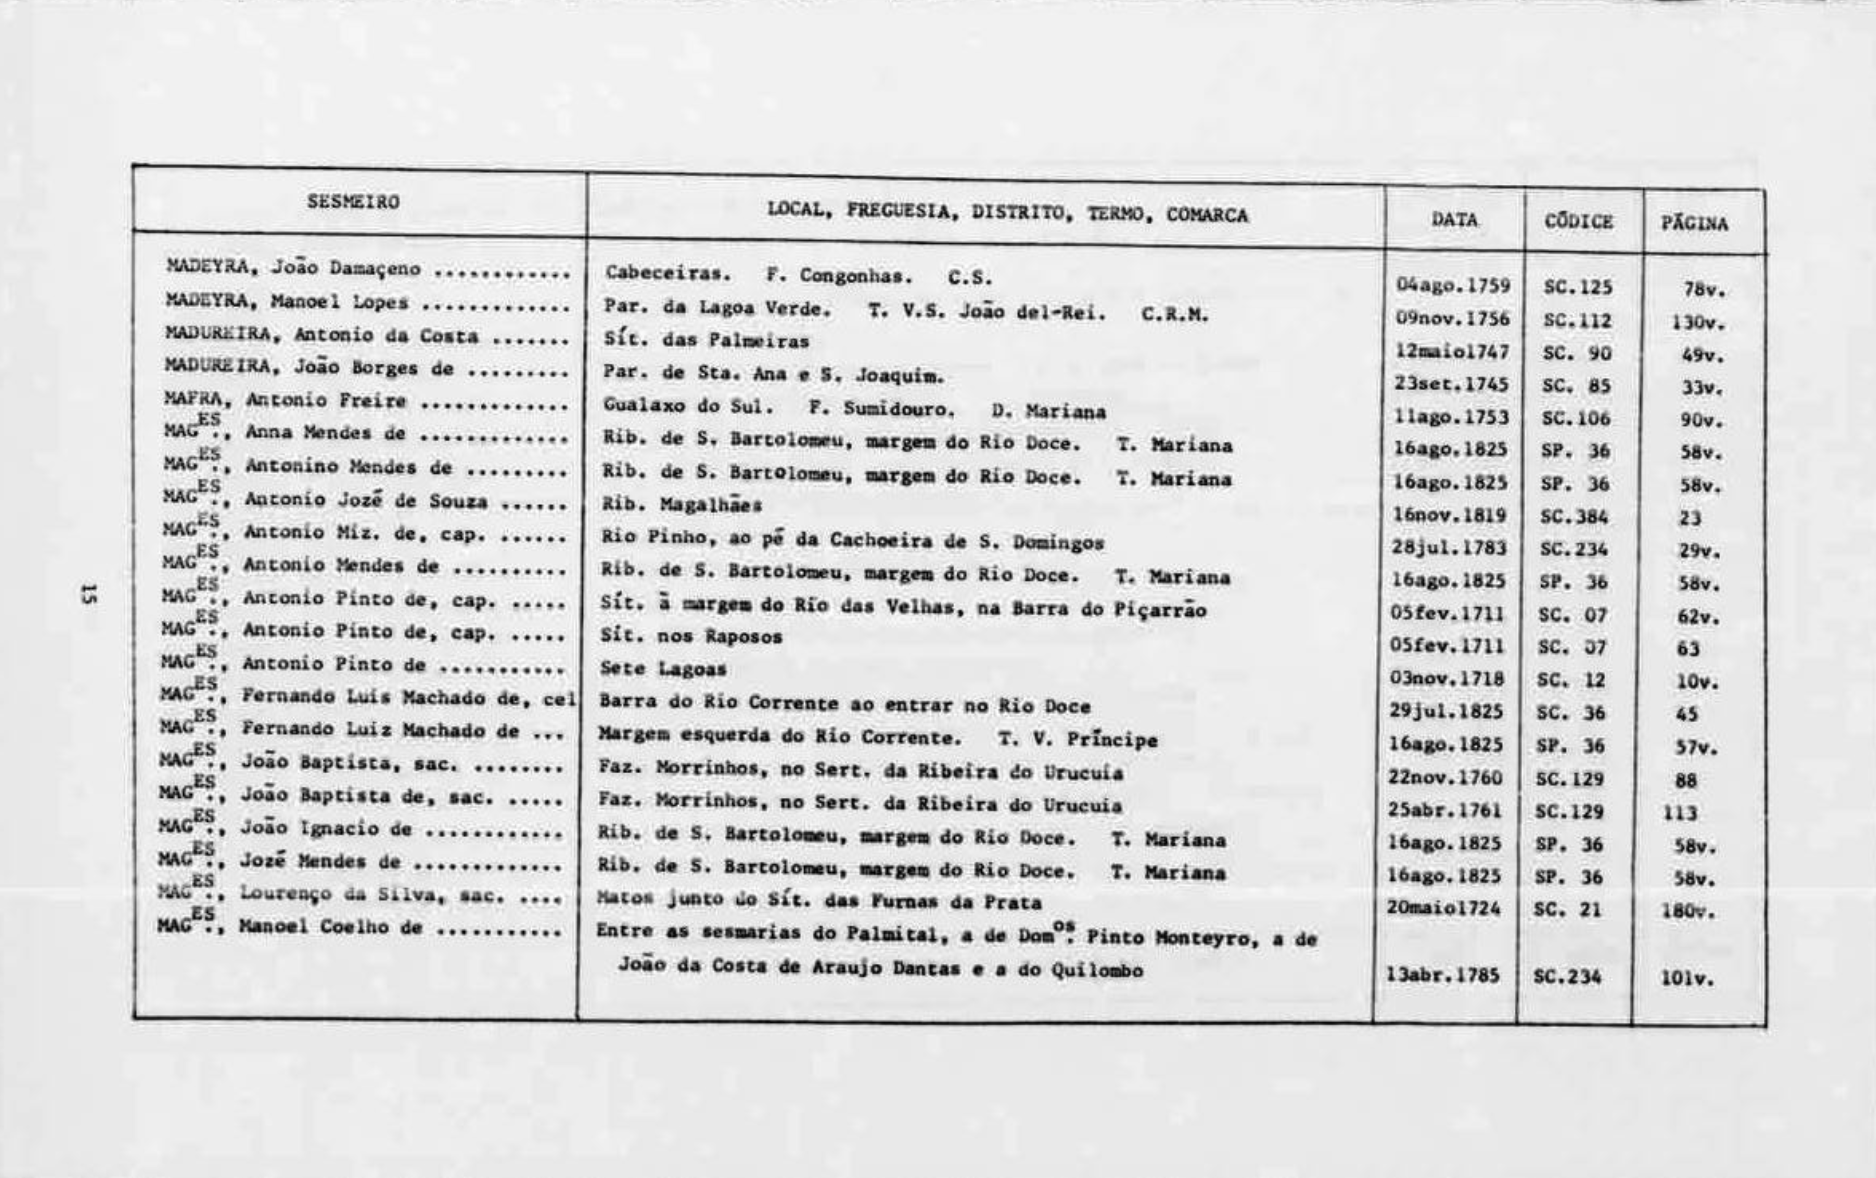
\includegraphics[width = \textwidth]{~/OneDrive - University of Illinois - Urbana/Research/Writing/git/Sesmarias/Pictures/minas_inventory.png}}
      \end{center}
      \textit{Notes:} Example of an inventory page for the state of Minas Gerais, obtained from   the Revista do Arquivo Publico Mineiro - Inventory of the sesmarias letters on the Public Archive Codex - Volume 37 (1988). Based on the letter we extract the name, the year, and the location of the grant.
  \end{figure}
  \end{landscape}

\clearpage

\begin{landscape}
\begin{figure}[htbp]
  \begin{center}
  \caption{Example original letter alongside its transcribed version}
  \label{fig:example_letter_other}
  \begin{subfigure}[b]{0.5\textwidth}
  \centering
  \vspace{-20cm}
  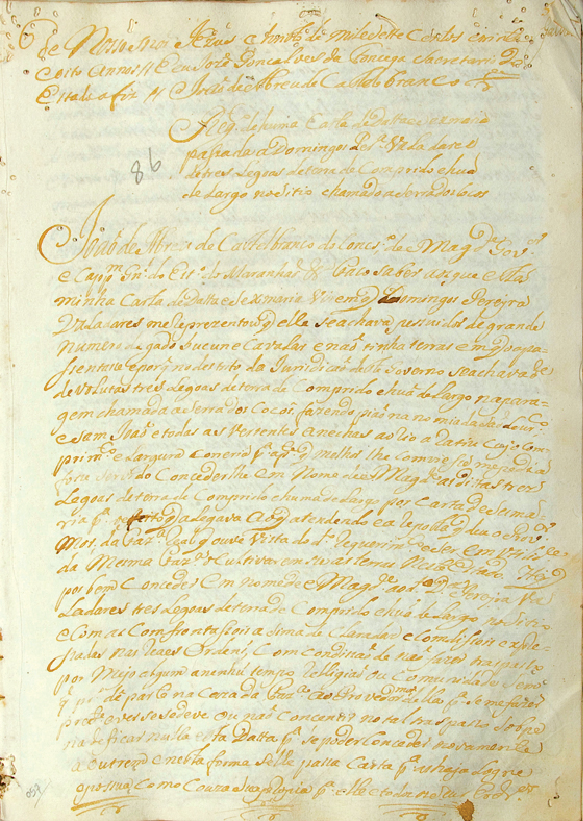
\includegraphics[width = \textwidth]
  {~/OneDrive - University of Illinois - Urbana/Research/Writing/git/Sesmarias/Pictures/0167f614a7c3b3fd38127f1545dbee7c.pdf}
  \end{subfigure}
  \begin{subfigure}[b]{0.6\textwidth}
  \centering
  %\vspace{-7.4cm}
  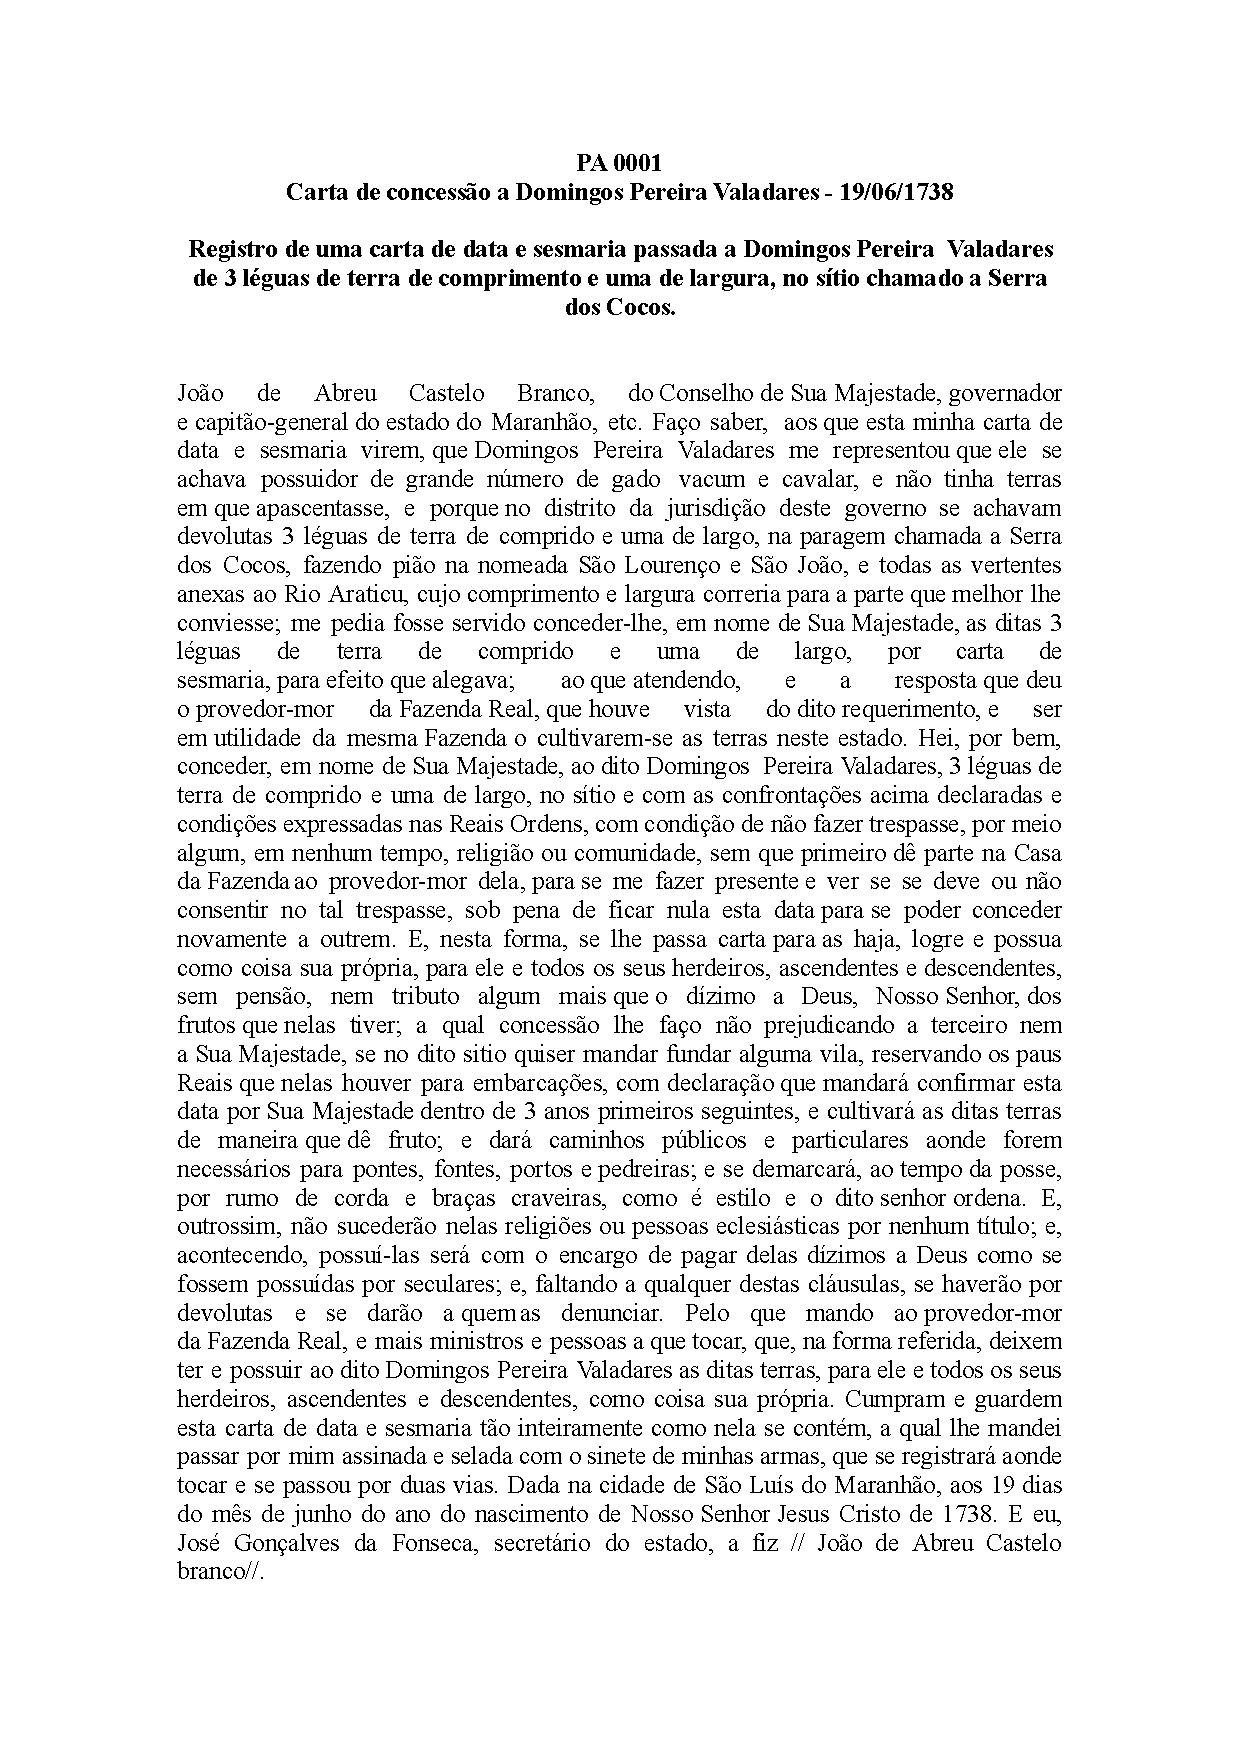
\includegraphics[page = 1, width = \textwidth]
  {~/OneDrive - University of Illinois - Urbana/Research/Writing/git/Sesmarias/Pictures/ea71ea6ac7c5ec3cefa24ded60ac6438.pdf}
  \end{subfigure}
  \end{center}
  \textit{Notes:} Example of an original manuscript (on the left) and its transcribed version (on the right). Obtained from \textit{SILB}.
\end{figure}
\end{landscape}

\clearpage

\begin{figure}[h!]
  \caption{Geographical distribution of Land Conflicts in Brazil}
  \begin{center}
     \makebox[\textwidth]			 
     {\includegraphics[width=0.9\paperwidth]{/Users/vinicius/Library/CloudStorage/OneDrive-UniversityofIllinois-Urbana/Research/Projects/JMP/02. Figures/00.Maps/cpt_conflict_data.png}}
  \end{center}
  \textit{Notes:} Geographical distribution of Land Conflicts in Brazil from 2014-2018 from the \textit{Comissao Pastoral da Terra} (Pastoral Comission of Land). Red dots indicate a conflict as reported on their yearly reports alongside with 2010 municipality boundaries.
  \label{fig:cpt_conflict}
\end{figure}

\begin{landscape}
  \begin{figure}
    \caption{Distribution of Land Grants in Minas Gerais and Sao Paulo alongside the Treaty of Tordesillas line}
    \begin{center}
       \makebox[\textwidth]			 
       {\includegraphics[width=0.85\paperwidth]{/Users/vinicius/Library/CloudStorage/OneDrive-UniversityofIllinois-Urbana/Research/Projects/JMP/02. Figures/00.Maps/sesmarias_tordesillas.png}}
    \end{center}
    \textit{Notes:} This figure shows the distribution of land grants in the states of Minas Gerais and Sao Paulo (shaded in gray) alongside the Treaty of Tordesillas. Black dots indicate the location of the land grants. The red vertical line is the Treaty of Tordesillas line following \textcite{Laudares2023-wl}. The treaty line is located at 48.7 W.
    \label{fig:Tordesillas}
  \end{figure}
  \end{landscape}
  
  \clearpage
  
  \begin{figure}
    \caption{Distribution of Land Grants alongside Bandeiras}
    \begin{center}
       \makebox[\textwidth]			 
       {\includegraphics[width=\paperwidth]{/Users/vinicius/Library/CloudStorage/OneDrive-UniversityofIllinois-Urbana/Research/Projects/JMP/02. Figures/00.Maps/sesmarias_bandeirantes.png}}
    \end{center}
    \textit{Notes:} This figure shows the distribution of the land grants alongside the \textit{bandeiras} routes. Each black dot represents a grant, while the red lines indicate the \textit{bandeiras}. Present-day state boundaries are shown.
    \label{fig:Bandeiras}
  \end{figure}
  
  \begin{figure}[h!]
    \caption{\textit{Bandeira} Routes and 1995 Municipalities}
    \begin{center}
       \makebox[\textwidth]			 
       {\includegraphics[width=\paperwidth]{/Users/vinicius/Library/CloudStorage/OneDrive-UniversityofIllinois-Urbana/Research/Projects/JMP/02. Figures/00.Maps/bandeiras_dist_SE.png}}
    \end{center}
    \textit{Notes:} Proximity to a \textit{Bandeira} route and 1995 municipalities boundaries in the states of Sao Paulo and Minas Gerais. Darker colors indicate that the municipality is close to a \textit{bandeira}, while lighter colors indicate that the municipality is further away. Yellow indicates any municipalities that are more than 50km from the explorer route. Red dots indicates the grants in those two states.
    \label{fig:bandeira_dist}
  \end{figure}
  
  \clearpage

\clearpage

\begin{figure}[h!]
  \caption{1872 Municipalities and Parish Locations}
  \begin{center}
     \makebox[\textwidth]			 
     {\includegraphics[width=\paperwidth]{/Users/vinicius/Library/CloudStorage/OneDrive-UniversityofIllinois-Urbana/Research/Projects/JMP/02. Figures/00.Maps/parishes_1872.png}}
  \end{center}
  \textit{Notes:} Geographical distribution of 1872 parishes alongside 1872 municipality and state boundaries. The states to which I have information on the land grants are highlighted in red. This map shows that several municipalities, especially in the Southeastern states have more than one parish per municipality. The sample increases by using parish-level information instead of municipalities from 337 to 815.
  \label{fig:parishes_1872}
\end{figure}

\clearpage

\begin{figure}[h!]
  \caption{Estimated Coefficients Excluding Municipalities Whose \% of Agricultural Units are above a cutoff}
  \begin{center}
     \makebox[\textwidth]			 
     {\includegraphics[width=0.8\paperwidth]{/Users/vinicius/Library/CloudStorage/OneDrive-UniversityofIllinois-Urbana/Research/Projects/JMP/02. Figures/00.Maps/robustness_cutoffs.png}}
  \end{center}
  \textit{Notes:} This figure shows the OLS results from \autoref{eqn:ols_matching_all} by excluding municipalities whose \% of farms over 2000ha is above a certain cutoff. For example, the estimate at 10 excludes all municipalities that have more than 10\% of their total agricultural land in farms over 2,000ha. Red line indicates the main estimate based on.
  \label{fig:robustness_cutoffs}
\end{figure}

\clearpage

% Marginal Distribution Effects:
\section*{Marginal Effects}


\begin{figure}[h!]
  \caption{Distributional Effects of the Grants}
  \centering
  \begin{subfigure}[b]{0.9\textwidth}
      \centering
      \includegraphics[width=\textwidth]
      {/Users/vinicius/Library/CloudStorage/OneDrive-UniversityofIllinois-Urbana/Research/Projects/JMP/02. Figures/00.Maps/different_cutoffs_marginal_all.png}
      \caption{Entire Sample}
  \end{subfigure}

  \hfill

  \begin{subfigure}[b]{0.9\textwidth}
      \centering
      \includegraphics[width=\textwidth]
      {/Users/vinicius/Library/CloudStorage/OneDrive-UniversityofIllinois-Urbana/Research/Projects/JMP/02. Figures/00.Maps/different_cutoffs_marginal_all_matched.png}
      \caption{Matched Sample}
  \end{subfigure}

  \justifying
  \noindent \textit{Notes:} This figure shows the estimates using \autoref{eqn:ols_matching} on the percentage of agricultural land in farms above a certain cutoff for both pre-1700 and post-1700 grants using the 1995 Agricultural Census. Figure (a), uses the entire sample, while Figure (b) uses the matched sample.
  \label{fig:all_marginal_cutoffs_full_sample}
\end{figure}

\clearpage

\begin{figure}[h!]
  \caption{Distribution Effects of the Grants - Northeastern States}
  \centering
  \begin{subfigure}[b]{0.9\textwidth}
      \centering
      \includegraphics[width=\textwidth]
      {/Users/vinicius/Library/CloudStorage/OneDrive-UniversityofIllinois-Urbana/Research/Projects/JMP/02. Figures/00.Maps/different_cutoffs_marginal_NE.png}
      \caption{Entire Sample}
  \end{subfigure}

  \hfill

  \begin{subfigure}[b]{0.9\textwidth}
      \centering
      \includegraphics[width=\textwidth]
      {/Users/vinicius/Library/CloudStorage/OneDrive-UniversityofIllinois-Urbana/Research/Projects/JMP/02. Figures/00.Maps/different_cutoffs_marginal_NE_matched.png}
      \caption{Matched Sample}
  \end{subfigure}

  \justifying
  \noindent \textit{Notes:} This figure shows the estimates using \autoref{eqn:ols_matching} on the percentage of agricultural land in farms above a certain cutoff for both pre-1700 and post-1700 grants on the Northeast states. Figure (a), uses the entire sample, while Figure (b) uses the matched sample.
  \label{fig:all_marginal_cutoffs_NE_sample}
\end{figure}

\clearpage

\begin{figure}[h!]
  \caption{Distributional Effects of the Grants - Southeastern States}
  \centering
  \begin{subfigure}[b]{0.9\textwidth}
      \centering
      \includegraphics[width=\textwidth]
      {/Users/vinicius/Library/CloudStorage/OneDrive-UniversityofIllinois-Urbana/Research/Projects/JMP/02. Figures/00.Maps/different_cutoffs_marginal_SE.png}
      \caption{Entire Sample}
  \end{subfigure}

  \hfill

  \begin{subfigure}[b]{0.9\textwidth}
      \centering
      \includegraphics[width=\textwidth]
      {/Users/vinicius/Library/CloudStorage/OneDrive-UniversityofIllinois-Urbana/Research/Projects/JMP/02. Figures/00.Maps/different_cutoffs_marginal_SE_matched.png}
      \caption{Matched Sample}
  \end{subfigure}

  \justifying
  \noindent \textit{Notes:} This figure shows the estimates using \autoref{eqn:ols_matching} on the percentage of agricultural land in farms above a certain cutoff for both pre-1700 and post-1700 grants on the Southeast states. Figure (a), uses the entire sample, while Figure (b) uses the matched sample.
  \label{fig:all_marginal_cutoffs_SE_sample}
\end{figure}

\clearpage

\section*{Share of Unproductive Land}

\begin{figure}[h!]
  \caption{Distributional Effects of the Grants}
  \centering
  \begin{subfigure}[b]{0.9\textwidth}
      \centering
      \includegraphics[width=\textwidth]
      {/Users/vinicius/Library/CloudStorage/OneDrive-UniversityofIllinois-Urbana/Research/Projects/JMP/02. Figures/00.Maps/unp_different_cutoffs_all.png}
      \caption{Entire Sample}
  \end{subfigure}

  \hfill

  \begin{subfigure}[b]{0.9\textwidth}
      \centering
      \includegraphics[width=\textwidth]
      {/Users/vinicius/Library/CloudStorage/OneDrive-UniversityofIllinois-Urbana/Research/Projects/JMP/02. Figures/00.Maps/unp_different_cutoffs_all_matched.png}
      \caption{Matched Sample}
  \end{subfigure}

  \justifying
  \noindent \textit{Notes:} This figure shows the estimates using \autoref{eqn:ols_matching} on the percentage of agricultural land in farms above a certain cutoff for both pre-1700 and post-1700 grants using the 1995 Agricultural Census. Figure (a), uses the entire sample, while Figure (b) uses the matched sample.
  \label{fig:unp_all_cutoffs_full_sample}
\end{figure}

\clearpage

\begin{figure}[h!]
  \caption{Distribution Effects of the Grants - Northeastern States}
  \centering
  \begin{subfigure}[b]{0.9\textwidth}
      \centering
      \includegraphics[width=\textwidth]
      {/Users/vinicius/Library/CloudStorage/OneDrive-UniversityofIllinois-Urbana/Research/Projects/JMP/02. Figures/00.Maps/unp_different_cutoffs_NE.png}
      \caption{Entire Sample}
  \end{subfigure}

  \hfill

  \begin{subfigure}[b]{0.9\textwidth}
      \centering
      \includegraphics[width=\textwidth]
      {/Users/vinicius/Library/CloudStorage/OneDrive-UniversityofIllinois-Urbana/Research/Projects/JMP/02. Figures/00.Maps/unp_different_cutoffs_NE_matched.png}
      \caption{Matched Sample}
  \end{subfigure}

  \justifying
  \noindent \textit{Notes:} This figure shows the estimates using \autoref{eqn:ols_matching} on the percentage of agricultural land in farms above a certain cutoff for both pre-1700 and post-1700 grants on the Northeast states. Figure (a), uses the entire sample, while Figure (b) uses the matched sample.
  \label{fig:unp_all_cutoffs_NE_sample}
\end{figure}

\clearpage

\begin{figure}[h!]
  \caption{Distribution Effects of the Grants - Southeastern States}
  \centering
  \begin{subfigure}[b]{0.9\textwidth}
      \centering
      \includegraphics[width=\textwidth]
      {/Users/vinicius/Library/CloudStorage/OneDrive-UniversityofIllinois-Urbana/Research/Projects/JMP/02. Figures/00.Maps/unp_different_cutoffs_SE.png}
      \caption{Entire Sample}
  \end{subfigure}

  \hfill

  \begin{subfigure}[b]{0.9\textwidth}
      \centering
      \includegraphics[width=\textwidth]
      {/Users/vinicius/Library/CloudStorage/OneDrive-UniversityofIllinois-Urbana/Research/Projects/JMP/02. Figures/00.Maps/unp_different_cutoffs_SE_matched.png}
      \caption{Matched Sample}
  \end{subfigure}

  \justifying
  \noindent \textit{Notes:} This figure shows the estimates using \autoref{eqn:ols_matching} on the percentage of agricultural land in farms above a certain cutoff for both pre-1700 and post-1700 grants on the Southeast states. Figure (a), uses the entire sample, while Figure (b) uses the matched sample.
  \label{fig:unp_all_cutoffs_SE_sample}
\end{figure}

% marginal effects

\clearpage


\begin{figure}[h!]
  \caption{Distributional Effects of the Grants}
  \centering
  \begin{subfigure}[b]{0.9\textwidth}
      \centering
      \includegraphics[width=\textwidth]
      {/Users/vinicius/Library/CloudStorage/OneDrive-UniversityofIllinois-Urbana/Research/Projects/JMP/02. Figures/00.Maps/unp_different_cutoffs_marginal_all.png}
      \caption{Entire Sample}
  \end{subfigure}

  \hfill

  \begin{subfigure}[b]{0.9\textwidth}
      \centering
      \includegraphics[width=\textwidth]
      {/Users/vinicius/Library/CloudStorage/OneDrive-UniversityofIllinois-Urbana/Research/Projects/JMP/02. Figures/00.Maps/unp_different_cutoffs_marginal_all_matched.png}
      \caption{Matched Sample}
  \end{subfigure}

  \justifying
  \noindent \textit{Notes:} This figure shows the estimates using \autoref{eqn:ols_matching} on the percentage of agricultural land in farms above a certain cutoff for both pre-1700 and post-1700 grants using the 1995 Agricultural Census. Figure (a), uses the entire sample, while Figure (b) uses the matched sample.
  \label{fig:unp_all_marginal_cutoffs_full_sample}
\end{figure}

\clearpage

\begin{figure}[h!]
  \caption{Distribution Effects of the Grants - Northeastern States}
  \centering
  \begin{subfigure}[b]{0.9\textwidth}
      \centering
      \includegraphics[width=\textwidth]
      {/Users/vinicius/Library/CloudStorage/OneDrive-UniversityofIllinois-Urbana/Research/Projects/JMP/02. Figures/00.Maps/unp_different_cutoffs_marginal_NE.png}
      \caption{Entire Sample}
  \end{subfigure}

  \hfill

  \begin{subfigure}[b]{0.9\textwidth}
      \centering
      \includegraphics[width=\textwidth]
      {/Users/vinicius/Library/CloudStorage/OneDrive-UniversityofIllinois-Urbana/Research/Projects/JMP/02. Figures/00.Maps/unp_different_cutoffs_marginal_NE_matched.png}
      \caption{Matched Sample}
  \end{subfigure}

  \justifying
  \noindent \textit{Notes:} This figure shows the estimates using \autoref{eqn:ols_matching} on the percentage of agricultural land in farms above a certain cutoff for both pre-1700 and post-1700 grants on the Northeast states. Figure (a), uses the entire sample, while Figure (b) uses the matched sample.
  \label{fig:unp_all_marginal_cutoffs_NE_sample}
\end{figure}

\clearpage

\begin{figure}[h!]
  \caption{Distributional Effects of the Grants - Southeastern States}
  \centering
  \begin{subfigure}[b]{0.9\textwidth}
      \centering
      \includegraphics[width=\textwidth]
      {/Users/vinicius/Library/CloudStorage/OneDrive-UniversityofIllinois-Urbana/Research/Projects/JMP/02. Figures/00.Maps/unp_different_cutoffs_marginal_SE.png}
      \caption{Entire Sample}
  \end{subfigure}

  \hfill

  \begin{subfigure}[b]{0.9\textwidth}
      \centering
      \includegraphics[width=\textwidth]
      {/Users/vinicius/Library/CloudStorage/OneDrive-UniversityofIllinois-Urbana/Research/Projects/JMP/02. Figures/00.Maps/unp_different_cutoffs_marginal_SE_matched.png}
      \caption{Matched Sample}
  \end{subfigure}

  \justifying
  \noindent \textit{Notes:} This figure shows the estimates using \autoref{eqn:ols_matching} on the percentage of agricultural land in farms above a certain cutoff for both pre-1700 and post-1700 grants on the Southeast states. Figure (a), uses the entire sample, while Figure (b) uses the matched sample.
  \label{fig:unp_all_marginal_cutoffs_SE_sample}
\end{figure}

\clearpage

% Livestock Area

\clearpage

\begin{landscape}
  \begin{figure}[htbp]
    \caption{Effects of Coastal Ban on Livestock with Varying Cutoffs on Livestock Area}
    \centering
    \begin{subfigure}[b]{0.65\textwidth}
        \centering
        \includegraphics[width=\textwidth]{/Users/vinicius/Library/CloudStorage/OneDrive-UniversityofIllinois-Urbana/Research/Projects/JMP/02. Figures/00.Maps/1995_Ag_Census_Coastal_All_Livestock_1600_Bands.png}
        \caption{Caption for Figure 1}
    \end{subfigure}
    \hfill
    \begin{subfigure}[b]{0.65\textwidth}
        \centering
        \includegraphics[width=\textwidth]{/Users/vinicius/Library/CloudStorage/OneDrive-UniversityofIllinois-Urbana/Research/Projects/JMP/02. Figures/00.Maps/1995_Ag_Census_Coastal_All_Livestock_1600_Bands_matched.png}
        \caption{Caption for Figure 2}
    \end{subfigure}

    \vspace{0.1cm} % adjust vertical spacing between rows

    \begin{subfigure}[b]{0.65\textwidth}
        \centering
        \includegraphics[width=\textwidth]{/Users/vinicius/Library/CloudStorage/OneDrive-UniversityofIllinois-Urbana/Research/Projects/JMP/02. Figures/00.Maps/1995_Ag_Census_Coastal_All_Livestock_1700_Bands.png}
        \caption{Caption for Figure 3}
    \end{subfigure}
    \hfill
    \begin{subfigure}[b]{0.65\textwidth}
        \centering
        \includegraphics[width=\textwidth]{/Users/vinicius/Library/CloudStorage/OneDrive-UniversityofIllinois-Urbana/Research/Projects/JMP/02. Figures/00.Maps/1995_Ag_Census_Coastal_All_Livestock_1700_Bands_matched.png}
        \caption{Caption for Figure 4}
    \end{subfigure}

    \vspace{0.5cm}
    \justifying
    \noindent \textit{Notes:} This figure shows the estimates using \autoref{eqn:livestock_1600} and \autoref{eqn:livestock_1700} on the share of agricultural land used for livestock production. Figures (a) and (b) show the differential effects for the Pre-1700 grants for the unmatched and matched sample respectively. Figures (c) and (d) show the same for the Post-1700 grants.
    \label{fig:robustness_all_distance_cutoff}
    
\end{figure}
\end{landscape}

\clearpage

\begin{landscape}
  \begin{figure}[htbp]
    \caption{Effects of Coastal Ban on Livestock with Varying Cutoffs on Livestock Area - Northeast Sample}
    \centering
    \begin{subfigure}[b]{0.65\textwidth}
        \centering
        \includegraphics[width=\textwidth]{/Users/vinicius/Library/CloudStorage/OneDrive-UniversityofIllinois-Urbana/Research/Projects/JMP/02. Figures/00.Maps/1995_Ag_Census_Coastal_NE_Livestock_1600_Bands.png}
        \caption{Caption for Figure 1}
        \label{fig:fig1}
    \end{subfigure}
    \hfill
    \begin{subfigure}[b]{0.65\textwidth}
        \centering
        \includegraphics[width=\textwidth]{/Users/vinicius/Library/CloudStorage/OneDrive-UniversityofIllinois-Urbana/Research/Projects/JMP/02. Figures/00.Maps/1995_Ag_Census_Coastal_NE_Livestock_1600_Bands_matched.png}
        \caption{Caption for Figure 2}
        \label{fig:fig2}
    \end{subfigure}

    \vspace{0.1cm} % adjust vertical spacing between rows

    \begin{subfigure}[b]{0.65\textwidth}
        \centering
        \includegraphics[width=\textwidth]{/Users/vinicius/Library/CloudStorage/OneDrive-UniversityofIllinois-Urbana/Research/Projects/JMP/02. Figures/00.Maps/1995_Ag_Census_Coastal_NE_Livestock_1700_Bands.png}
        \caption{Caption for Figure 3}
        \label{fig:fig3}
    \end{subfigure}
    \hfill
    \begin{subfigure}[b]{0.65\textwidth}
        \centering
        \includegraphics[width=\textwidth]{/Users/vinicius/Library/CloudStorage/OneDrive-UniversityofIllinois-Urbana/Research/Projects/JMP/02. Figures/00.Maps/1995_Ag_Census_Coastal_NE_Livestock_1700_Bands_matched.png}
        \caption{Caption for Figure 4}
        \label{fig:fig4}
    \end{subfigure}

    \vspace{0.5cm}
    \justifying
    \noindent \textit{Notes:} This figure shows the estimates using \autoref{eqn:livestock_1600} and \autoref{eqn:livestock_1700} on the share of agricultural land used for livestock production for the Northeast sample. Figures (a) and (b) show the differential effects for the Pre-1700 grants for the unmatched and matched sample respectively. Figures (c) and (d) show the same for the Post-1700 grants.
    \label{fig:robustness_NE_distance_cutoff}
    
\end{figure}
\end{landscape}

\clearpage

\begin{landscape}
  \begin{figure}[htbp]
    \caption{Effects of Coastal Ban on Livestock with Varying Cutoffs on Livestock Area - Southeast Sample}
    \centering
    \begin{subfigure}[b]{0.65\textwidth}
        \centering
        \includegraphics[width=\textwidth]{/Users/vinicius/Library/CloudStorage/OneDrive-UniversityofIllinois-Urbana/Research/Projects/JMP/02. Figures/00.Maps/1995_Ag_Census_Coastal_SE_Livestock_1600_Bands.png}
        \caption{Caption for Figure 1}
        \label{fig:fig1}
    \end{subfigure}
    \hfill
    \begin{subfigure}[b]{0.65\textwidth}
        \centering
        \includegraphics[width=\textwidth]{/Users/vinicius/Library/CloudStorage/OneDrive-UniversityofIllinois-Urbana/Research/Projects/JMP/02. Figures/00.Maps/1995_Ag_Census_Coastal_SE_Livestock_1600_Bands_matched.png}
        \caption{Caption for Figure 2}
        \label{fig:fig2}
    \end{subfigure}

    \vspace{0.1cm} % adjust vertical spacing between rows

    \begin{subfigure}[b]{0.65\textwidth}
        \centering
        \includegraphics[width=\textwidth]{/Users/vinicius/Library/CloudStorage/OneDrive-UniversityofIllinois-Urbana/Research/Projects/JMP/02. Figures/00.Maps/1995_Ag_Census_Coastal_SE_Livestock_1700_Bands.png}
        \caption{Caption for Figure 3}
        \label{fig:fig3}
    \end{subfigure}
    \hfill
    \begin{subfigure}[b]{0.65\textwidth}
        \centering
        \includegraphics[width=\textwidth]{/Users/vinicius/Library/CloudStorage/OneDrive-UniversityofIllinois-Urbana/Research/Projects/JMP/02. Figures/00.Maps/1995_Ag_Census_Coastal_SE_Livestock_1700_Bands_matched.png}
        \caption{Caption for Figure 4}
        \label{fig:fig4}
    \end{subfigure}

    \vspace{0.5cm}
    \justifying
    \noindent \textit{Notes:} This figure shows the estimates using \autoref{eqn:livestock_1600} and \autoref{eqn:livestock_1700} on the share of agricultural land used for livestock production for the Southeast sample. Figures (a) and (b) show the differential effects for the Pre-1700 grants for the unmatched and matched sample respectively. Figures (c) and (d) show the same for the Post-1700 grants.
    \label{fig:robustness_SE_distance_cutoff}
    
\end{figure}
\end{landscape}

\clearpage 

% Over 2,000ha 

\begin{landscape}
  \begin{figure}[htbp]
    \centering
    \caption{Effects of Coastal Ban with Varying Cutoffs on Agricultural Land on Properties over 2,000ha}
    \begin{subfigure}[b]{0.65\textwidth}
        \centering
        \includegraphics[width=\textwidth]{/Users/vinicius/Library/CloudStorage/OneDrive-UniversityofIllinois-Urbana/Research/Projects/JMP/02. Figures/00.Maps/1995_Ag_Census_Coastal_All_2000ha_1600_Bands.png}
        \caption{Caption for Figure 1}
        \label{fig:fig1}
    \end{subfigure}
    \hfill
    \begin{subfigure}[b]{0.65\textwidth}
        \centering
        \includegraphics[width=\textwidth]{/Users/vinicius/Library/CloudStorage/OneDrive-UniversityofIllinois-Urbana/Research/Projects/JMP/02. Figures/00.Maps/1995_Ag_Census_Coastal_All_2000ha_1600_Bands_matched.png}
        \caption{Caption for Figure 2}
        \label{fig:fig2}
    \end{subfigure}

    \vspace{0.1cm} % adjust vertical spacing between rows

    \begin{subfigure}[b]{0.65\textwidth}
        \centering
        \includegraphics[width=\textwidth]{/Users/vinicius/Library/CloudStorage/OneDrive-UniversityofIllinois-Urbana/Research/Projects/JMP/02. Figures/00.Maps/1995_Ag_Census_Coastal_All_2000ha_1700_Bands.png}
        \caption{Caption for Figure 3}
        \label{fig:fig3}
    \end{subfigure}
    \hfill
    \begin{subfigure}[b]{0.65\textwidth}
        \centering
        \includegraphics[width=\textwidth]{/Users/vinicius/Library/CloudStorage/OneDrive-UniversityofIllinois-Urbana/Research/Projects/JMP/02. Figures/00.Maps/1995_Ag_Census_Coastal_All_2000ha_1700_Bands_matched.png}
        \caption{Caption for Figure 4}
        \label{fig:fig4}
    \end{subfigure}

    \vspace{0.5cm}
    \justifying
    \noindent \textit{Notes:} This figure shows the estimates using \autoref{eqn:livestock_1600} and \autoref{eqn:livestock_1700} on the share of agricultural land used in properties over 2,000ha. Figures (a) and (b) show the differential effects for the Pre-1700 grants for the unmatched and matched sample respectively. Figures (c) and (d) show the same for the Post-1700 grants.
    \label{fig:robustness_all_landsize_distance_cutoff}
    
\end{figure}
\end{landscape}

\clearpage

\begin{landscape}
  \begin{figure}[htbp]
    \centering
    \caption{Effects of Coastal Ban with Varying Cutoffs on Agricultural Land on Properties over 2,000ha - Northeast samples}
    \begin{subfigure}[b]{0.65\textwidth}
        \centering
        \includegraphics[width=\textwidth]{/Users/vinicius/Library/CloudStorage/OneDrive-UniversityofIllinois-Urbana/Research/Projects/JMP/02. Figures/00.Maps/1995_Ag_Census_Coastal_NE_2000ha_1600_Bands.png}
        \caption{Caption for Figure 1}
        \label{fig:fig1}
    \end{subfigure}
    \hfill
    \begin{subfigure}[b]{0.65\textwidth}
        \centering
        \includegraphics[width=\textwidth]{/Users/vinicius/Library/CloudStorage/OneDrive-UniversityofIllinois-Urbana/Research/Projects/JMP/02. Figures/00.Maps/1995_Ag_Census_Coastal_NE_2000ha_1600_Bands_matched.png}
        \caption{Caption for Figure 2}
        \label{fig:fig2}
    \end{subfigure}

    \vspace{0.1cm} % adjust vertical spacing between rows

    \begin{subfigure}[b]{0.65\textwidth}
        \centering
        \includegraphics[width=\textwidth]{/Users/vinicius/Library/CloudStorage/OneDrive-UniversityofIllinois-Urbana/Research/Projects/JMP/02. Figures/00.Maps/1995_Ag_Census_Coastal_NE_2000ha_1700_Bands.png}
        \caption{Caption for Figure 3}
        \label{fig:fig3}
    \end{subfigure}
    \hfill
    \begin{subfigure}[b]{0.65\textwidth}
        \centering
        \includegraphics[width=\textwidth]{/Users/vinicius/Library/CloudStorage/OneDrive-UniversityofIllinois-Urbana/Research/Projects/JMP/02. Figures/00.Maps/1995_Ag_Census_Coastal_NE_2000ha_1700_Bands_matched.png}
        \caption{Caption for Figure 4}
        \label{fig:fig4}
    \end{subfigure}

    \vspace{0.5cm}
    \justifying
    \noindent \textit{Notes:} This figure shows the estimates using \autoref{eqn:livestock_1600} and \autoref{eqn:livestock_1700} on the share of agricultural land used in properties over 2,000h for the Northeast sample. Figures (a) and (b) show the differential effects for the Pre-1700 grants for the unmatched and matched sample respectively. Figures (c) and (d) show the same for the Post-1700 grants.
    \label{fig:robustness_NE_landsize_distance_cutoff}
    
\end{figure}
\end{landscape}

\clearpage

\begin{landscape}
  \begin{figure}[htbp]
    \centering
    \caption{Effects of Coastal Ban with Varying Cutoffs on Agricultural Land on Properties over 2,000ha - Southeast Sample}
    \begin{subfigure}[b]{0.65\textwidth}
        \centering
        \includegraphics[width=\textwidth]{/Users/vinicius/Library/CloudStorage/OneDrive-UniversityofIllinois-Urbana/Research/Projects/JMP/02. Figures/00.Maps/1995_Ag_Census_Coastal_SE_2000ha_1600_Bands.png}
        \caption{Caption for Figure 1}
        \label{fig:fig1}
    \end{subfigure}
    \hfill
    \begin{subfigure}[b]{0.65\textwidth}
        \centering
        \includegraphics[width=\textwidth]{/Users/vinicius/Library/CloudStorage/OneDrive-UniversityofIllinois-Urbana/Research/Projects/JMP/02. Figures/00.Maps/1995_Ag_Census_Coastal_SE_2000ha_1600_Bands_matched.png}
        \caption{Caption for Figure 2}
        \label{fig:fig2}
    \end{subfigure}

    \vspace{0.1cm} % adjust vertical spacing between rows

    \begin{subfigure}[b]{0.65\textwidth}
        \centering
        \includegraphics[width=\textwidth]{/Users/vinicius/Library/CloudStorage/OneDrive-UniversityofIllinois-Urbana/Research/Projects/JMP/02. Figures/00.Maps/1995_Ag_Census_Coastal_SE_2000ha_1700_Bands.png}
        \caption{Caption for Figure 3}
        \label{fig:fig3}
    \end{subfigure}
    \hfill
    \begin{subfigure}[b]{0.65\textwidth}
        \centering
        \includegraphics[width=\textwidth]{/Users/vinicius/Library/CloudStorage/OneDrive-UniversityofIllinois-Urbana/Research/Projects/JMP/02. Figures/00.Maps/1995_Ag_Census_Coastal_SE_2000ha_1700_Bands_matched.png}
        \caption{Caption for Figure 4}
        \label{fig:fig4}
    \end{subfigure}

    \vspace{0.5cm}
    \justifying
    \noindent \textit{Notes:} This figure shows the estimates using \autoref{eqn:livestock_1600} and \autoref{eqn:livestock_1700} on the share of agricultural land used in properties over 2,000ha for the Southeast sample. Figures (a) and (b) show the differential effects for the Pre-1700 grants for the unmatched and matched sample respectively. Figures (c) and (d) show the same for the Post-1700 grants.
    \label{fig:robustness_SE_landsize_distance_cutoff}
    
\end{figure}
\end{landscape}

\clearpage 

% Other stuff

\begin{figure}[h!]
  \caption{Estimated Coefficients Excluding Municipalities Whose \% of Agricultural Units are above a cutoff \label{fig:iv_1995_bandeira_dist}}
  \begin{center}
     \makebox[\textwidth]			 
     {\includegraphics[width=0.8\paperwidth]{/Users/vinicius/Library/CloudStorage/OneDrive-UniversityofIllinois-Urbana/Research/Projects/JMP/02. Figures/00.Maps/iv_robustness_cutoffs.png}}
  \end{center}
  \textit{Notes:} Figure shows the estimates from \autoref{eqn:ivequation} by excluding municipalities too far from a certain cutoff. For example, the first estimate at 50 indicates that the sample selection are only municipalities within 50km of a \textit{bandeira}. 95\% confidence intervals are represented as error bars. Red line indicates the main estimate reported in Column 2 of \autoref{tab:iv_all_sizes_1995}.
  \label{fig:iv_robustness_cutoffs}
\end{figure}

\clearpage

\begin{figure}[h!]
    \caption{\textit{Bandeira} Routes and 1995 Municipalities}
    \begin{center}
       \makebox[\textwidth]			 
       {\includegraphics[width=0.75\paperwidth]{/Users/vinicius/Library/CloudStorage/OneDrive-UniversityofIllinois-Urbana/Research/Projects/JMP/02. Figures/00.Maps/1995_IV_distance_first_stage.png}}
    \end{center}
    \textit{Notes:} Binscatter plot showing the correlation between proximity to a \textit{Bandeira} route and the probability of having received a land grant. Each observation is a 1995 municipality from the states of Sao Paulo and Minas Gerais.
    \label{fig:bandeira_dist_graph}
  \end{figure}
  
  \clearpage

\begin{figure}
  \caption{Robustness checks on the IV estimates for the percentage of farms over 2,000 ha}
  \begin{center}
     \makebox[\textwidth]			 
     {\includegraphics[width=0.9\paperwidth]{/Users/vinicius/Library/CloudStorage/OneDrive-UniversityofIllinois-Urbana/Research/Projects/JMP/02. Figures/00.Maps/ivDiag_1995.png}}
  \end{center}
  \textit{Notes:} Figure shows the OLS and IV estimators, alongside a variety of robustness checks for both which include bootstrapped standard errors, Anderson-Rubin Confidence intervals \protect\parencite{Anderson1949-aa}, and tF Confidence Intervals \protect\parencite{Lee2022-jw}. Confidence intervals shown are at the 95\% level.
  \label{fig:ivdiag_1995}
\end{figure}

\clearpage

\input{~/OneDrive - University of Illinois - Urbana/Research/Projects/JMP/03. Tables/1995_Geographical_Balance_Year_Split.tex}

\clearpage

\input{~/OneDrive - University of Illinois - Urbana/Research/Projects/JMP/03. Tables/1995_Ag_Census_Land_Size_Varying.tex}

\clearpage

\input{~/OneDrive - University of Illinois - Urbana/Research/Projects/JMP/03. Tables/1995_Ag_Census_Livestock_Coastal_NE.tex}

\clearpage

\input{~/OneDrive - University of Illinois - Urbana/Research/Projects/JMP/03. Tables/1995_Ag_Census_Livestock_Coastal_SE.tex}

\clearpage

\input{~/OneDrive - University of Illinois - Urbana/Research/Projects/JMP/03. Tables/1995_Ag_Census_Land_Inequality_Coastal_NE.tex}

\clearpage

\input{~/OneDrive - University of Illinois - Urbana/Research/Projects/JMP/03. Tables/1995_Ag_Census_Land_Inequality_Coastal_SE.tex}

\clearpage

\input{~/OneDrive - University of Illinois - Urbana/Research/Projects/JMP/03. Tables/1995_First_Stage_Year.tex}

\clearpage

\input{~/OneDrive - University of Illinois - Urbana/Research/Projects/JMP/03. Tables/1995_IV_All_Lands_1700.tex}

\clearpage

\subsection*{1970 Census}

\input{~/OneDrive - University of Illinois - Urbana/Research/Projects/JMP/03. Tables/1970_Census_Matching_All.tex}

\input{~/OneDrive - University of Illinois - Urbana/Research/Projects/JMP/03. Tables/1970_Census_Matching_NE_All.tex}

\input{~/OneDrive - University of Illinois - Urbana/Research/Projects/JMP/03. Tables/1970_Census_Matching_SE_All.tex}


\subsection{1980 Census}

\input{~/OneDrive - University of Illinois - Urbana/Research/Projects/JMP/03. Tables/1980_Census_Race.tex}

\begin{comment}
\subsection{1991 Census}
\end{comment}


\section{Data Source Appendix}
\label{app:data_source_appendix}

Below I describe the sources to which the land grants were compiled from. The states with a $^*$ indicate that the data collection was done by the researchers at SILB.

\vspace{2mm}

\textbf{Pernambuco$^*$}
\begin{itemize}
\item Documentação Histórica Pernambucana. Recife: Imprensa Oficial, 1954. Vol. 1-2
\item Documentação Histórica Pernambucana: sesmarias. Recife: Secretaria de Educação e Cultura. Biblioteca Pública, 1959. Vol. 1-4
\item Coleção Documentos Históricos Biblioteca Nacional do Rio de Janeiro. Vol. 20-22
\item Arquivo Nacional do Rio de Janeiro. Códice 427
\item Arquivo Nacional do Rio de Janeiro. Códice 155
\item Livro do Tombo do Mosteiro de São Bento de Olinda, Imprensa Oficial - Recife, 1948
\item Livros do Tombo de São Bento. Book 1-3
\item Revista do Instituto Arqueológico, Histórico e Geográfico Pernambucano, 1896.
\item Revista do Instituto Histórico de Goiana, 1871.
\end{itemize}

\textbf{Rio Grande do Norte$^*$}
\begin{itemize}
  \item O Treslado do auto e mais diligências que se fizeram sobre as datas de terras da capitania do Rio Grande, que se tinham dado. Fortaleza: Revista do Instituto do Ceará, 1909, Ano XXIII.
  \item IHGRN - Fundo Sesmarias - Books 1-9
  \item Documentos Históricos da Biblioteca Nacional do Rio de Janeiro..Vol. 23
  \item Documentos Históricos da Biblioteca Nacional do Rio de Janeiro..Vol. 24 Arquivo Nacional Rio de Janeiro, Códice 427
\end{itemize}

\begin{comment}
\textbf{Ceara}
\begin{itemize}
  \item 
\end{itemize}
\end{comment}

\clearpage

\textbf{Bahia$^*$}
\begin{itemize}
  \item Códice 427 - Rio de Janeiro
  \item FREIRE, Felisbello. História territorial do Brasil. Salvador: Secretaria da Cultura e Turismo, Instituto Geográfico e Histórico da Bahia, 1998
  \item DHBN - cartas publicadas na coleção Documentos Históricos da Biblioteca Nacional - DHBN, volumes 13 a 22
  \item  Anais do Arquivo Público do Estado da Bahia - Publicação dos anais do APEB - Anais do Arquivo Público do Estado da Bahia. Volumes 3 e 11
  \item Códice 155 - Rio de Janeiro
  \item Mosteiro de São Bento - Cartas publicadas nos Livros do Tombo do Mosteiro de São Bento  
\end{itemize}

\textbf{Paraiba$^*$}
\begin{itemize}
  \item British Library: Livro 1 (Land Grants (sesmarias) / Land Registers, 1757 - 1764); Livro 2: (Plots of Land 1722-1727 / Land Grants (sesmarias) 1722-1727); Livro 3: (Land Grants (sesmarias), 1785 -1787); Livro 4: (Land Grants (sesmarias), 1728 -1738); Livro 5: (Land Grants (sesmarias), 1816 - 1824); Livro 6: (Land Grants (sesmarias), 1747 - 1755); Livro 7: (Land Grants (sesmarias), 1789 - 1808); Livro 8: (Plots of Land - 1714-1717 / Land grants (sesmarias); Livro 9: (Land Grant - Various Parishes, 1768 - 1776); Livro 10: (Land Grants 1704-1722 / Sesmarias 1704-1722)
  \item TAVARES, João de Lira. Apontamentos para a História territorial da Parahyba. ed. Facsimilar. Brasília: Senado Federal, 1982. vol. CCXLV.
  \item Documentação Histórica Pernambucana: sesmarias. Recife:
  \item SECRETARIA DE EDUCAÇÃO E CULTURA BIBLIOTECA PÚBLICA, 1959
  \item Documentos Históricos da Biblioteca Nacional (DHBN): DHBN, V. 23. P.402-405.
  \item Códice 427 - Arquivo Nacional - Rio de Janeiro
  PUBLICAÇÕES DO ARCHIVO NACIONAL. VOL XXVII RIO DE
  JANEIRO Officinas Graphicas do ARCHIVO NACIONAL 1931. (Códice 155)
  \item Biblioteca Pública do Estado de Pernambuco (BPE) - Recife
  
\end{itemize}


\textbf{Sao Paulo}
\begin{itemize}
\item \textcite{noauthor_1921-qd} Vols. 1-3 
\item \textcite{Instituto-Historico-e-Geografico-de-Sao-Paulo1928-ej}
\end{itemize}

\textbf{Minas Gerais}
\begin{itemize}
  \item Revista do Arquivo Publico Mineiro - Inventory of the sesmarias letters on the Public Archive Codex - Volume 37 (1988)
  \item Revista do Arquivo Publico Mineiro - Volumes 10-24 (1905-1933). 
\end{itemize}

\clearpage

\section{Description of Letters and Georeferencing}
\label{app:appendix_data}

Below is a description on how the process used to georeference the land grants.

\begin{enumerate}
  \item Based on the letter information, since a location was required for the land to be granted, the geographical information on where the land was requested and who their neighbors was extracted.
  %\item For example, the sesmaria of 
  \item It is also possible to georeference based on the person's neighbors. 
  \begin{enumerate}
    \item For example, the sesmaria of Matheus Ferndandes Ramos, granted in 1698, is described as being close to the sesmaria of Lucas Pedroso, granted in 1638. 
  \end{enumerate}
  \item When not possible to georeference based on the above, the location is approximated at the municipality level. 
\end{enumerate}

An example on how the georeferencing process was done for the [...]

\begin{enumerate}
    \item First, the geographical landmarks in the text are identified.
    \begin{figure}[h!]
        \begin{center}
        \vspace{3mm}
        \makebox[\textwidth]	
        {\includegraphics[width = 0.5\textwidth]{~/OneDrive - University of Illinois - Urbana/Research/Writing/git/Sesmarias/GR_Pics/text.png}}
        \end{center}
    \end{figure}
    \begin{itemize}
        \item \textit{Campos de Ytacurubitiva} (Fields of Ytacurubitiva) $\rightarrow$ Same as Itaquaquecetuba (Costa, 2021).
        \item Boigi Mirim $\rightarrow$ Municipality of Mogi das Cruzes (Leme, 2014).
        \item Rio Grande de Anhemby $\rightarrow$ Tiete River (Vilardaga, 2020).
        \item Rio Guyao $\rightarrow$ Guaio River.
    \end{itemize}
    \item Based on the landmarks, it is possible to approximate the location of the grant in the following location. The are is currently a rich area of the city of Sao Paulo.
    \begin{figure}[h!]
        \begin{center}
        \vspace{3mm}
        \makebox[\textwidth]	
        {\includegraphics[width = 0.55\textwidth]{~/OneDrive - University of Illinois - Urbana/Research/Writing/git/Sesmarias/GR_Pics/georeferencing.png}}
        \end{center}
    \end{figure}  

    \centering
    \textbf{Coordinates:} (-46.3, -23.5)
\end{enumerate}

%Additionally, here are three practical examples on how each was georeferenced: 

\clearpage

\section{Parish Level Georeferencing}
\label{app:georeferencing_parishes}

The 1872 census was conducted at the parish level. For the 1872 census, the seven states that had a total of 337 municipalities, I georeferenced the information at the parish level for that census, increasing the total sample size to 881.

Below is a description of how the georeferencing was done:

\begin{enumerate}
  \item If the municipalities only had one parish, then the parish location is the same as the municipality seat.
  \begin{enumerate}
    \item The municipality of Serpa in Amazonas has only one parish, ``Nossa Senhora do Rosário de Serpa", therefore, it is georeferenced to the municipality seat of Serpa.
  \end{enumerate}
  \item If a municipality has more than one parish, first, I checked based on the name whether or not the parish level can be traced to a present-day city.
  \begin{enumerate}
    \item The municipality of Vigia in Para has three parishes: ``Nossa Senhora de Nazaré da Vigia", ``Nossa Senhora do Rosário de Collares'', and ``São Caetano de Odivellas''. 
    \item All of these parishes can be traced down to present-day cities, ``Nossa Senhora de Nazaré da Vigia'' is the present-day municipality of Vigia, ``Nossa Senhora do Rosário de Collares'' is the present-day municipality of Collares, and ``São Caetano de Odivellas'' is the present-day municipality of São Caetano de Odivellas
  \end{enumerate}
  \item If the parish cannot be traced down based on the name of a present-day municipality then I looked at other sources.\footnote{https://cidades.ibge.gov.br/ includes information on historical names for municipalities, based on their history.}
\end{enumerate}

\clearpage

%\section{Coastal RDD - Results}
%\label{app:coastal_rdd}
%Given the setting of the coastal ban I estimate the following set of equations:
%\begin{equation}
%  Y_{m,s} = \beta \cdot CoastDist_{m,s} + f(D_{m,s})+ \mu_s + X_{m,s} + \epsilon_{m,s}
%\end{equation}

%For the 1970-2010 census, given that I have information at the individual level I estimate:
%\begin{equation}
%  Y_{i,m,s} = \beta \cdot CoastDist_{m} + f(D_{m})+ \mu_s + X_{i,m,s} + \epsilon_{i,m,s}
%\end{equation}

\begin{comment}
\section{Data Appendix - 1872}
\label{app:variable_construction_1872}

Below are the definitions of the variables measured for the 1872 census and how they were constructed. Some of the variables are already defined in the census:

\subsection{Base Variables, available by gender and free vs. enslaved:}

\begin{enumerate}
  \item Number of Literate People
  \item Number of People 6-15 Attending/Not Attending/No Information on Schooling
  \item Demographic Information on Race
    \begin{enumerate}
      \item Number of Enslaved People
      \item Number of Pardos
      \item Number of Whites
      \item Number of Blacks
      \item Number of Caboclos
    \end{enumerate}
  \item Number of People not born in the state based on origin: Within Brazil or from another country.
  \item Number of people on types of jobs: Liberal/Manual/Agricultural/Industry/Other Jobs/No Jobs
    \begin{enumerate}
      \item Liberal: Religious men/women, judges, lawyers, notaries, attorneys, justice officials, medics, surgeons, pharmacists, midwives, teachers, public officials, and artists.
      \item Manual or Mechanical: 
      \item Agricultural: Farmers and livestock breeders.
      \item Industry: Manufacturers and merchants.
      \item Other: Military officers, mariners, fishermen, capitalists/owners, \textit{jornaleiros} (workers that are paid based on a working day), domestic workers, and no information
    \end{enumerate}
  \item Number of people by age group.
\end{enumerate}

\subsection{Constructed Variables:}

\begin{enumerate}
  \item Proportion of Slaves to Free Population:
  $$ 100 \times \frac{\text{\# of Enslaved People}}{\text{\# of Free People}} $$

  \item Proportion of Slaves in Agriculture:
  $$ 100 \times \frac{\text{\# of Slaves in Agriculture}}{\text{\# of Slaves}}$$

\end{enumerate}
\end{comment}

\end{document}